\documentclass[superscriptaddress, amsmath, amssymb, aps, pre, floatfix]{revtex4-2}

\makeatletter
\NewCommandCopy\@@pmod\pmod
\DeclareRobustCommand{\pmod}{\@ifstar\@pmods\@@pmod}
\def\@pmods#1{\mkern4mu({\operator@font mod}\mkern 6mu#1)}
\makeatother


\synctex=1 

\usepackage[utf8]{inputenc}
\usepackage[T1]{fontenc}
\usepackage{graphicx}
% \usepackage{showframe}
\usepackage{tcolorbox}
\usepackage{grffile}
\usepackage{fixme}
\usepackage{float}
\usepackage{longtable}
\usepackage{wrapfig}
\usepackage{rotating}
\usepackage[normalem]{ulem}
\usepackage{amsmath}
\usepackage[outline]{contour}
\usepackage{textcomp}
\usepackage{amssymb}
\usepackage{xfrac}
\usepackage{capt-of}
\usepackage{hyperref}
\hypersetup{hidelinks}
\usepackage{placeins}
\usepackage{xr}

\usepackage{algpseudocode}
\usepackage{pgfplots}
\usepackage{pgfplotstable}
\usepackage{relsize}
\usepackage[export]{adjustbox}
\usepackage{lipsum}

\usepackage{customcolours}
\providecommand{\varv}{v}
\providecommand{\acos}{}
\providecommand{\tr}{}
\providecommand{\mdet}[1]{}
\providecommand{\abs}[1][]{}
\providecommand{\dmat}{}
\usepackage{customcommands}
\usepackage{globalplotconfig}

\usepackage{bm}
\usepackage{standalone}
\usepackage{tikz}
\newtcolorbox{mybox}[1]{colback=bright_red!5!,colframe=white!0, fonttitle=\bfseries,title=#1}

\usepackage{ifthen}

\usepackage{pgfmath}
\usepackage{pgfplots}
\usepackage{todonotes}
\newcommand*{\Scale}[2][4]{\scalebox{#1}{$#2$}}%
\newcommand*{\Resize}[2]{\resizebox{#1}{!}{$#2$}}%

\usepackage{xfp}


% \usepackage{xparse}
\usepackage{dsfont}
%\usepackage{amsmath}
%\usepackage{amssymb}
\usepackage{dsfont}
\usepackage{relsize}

% \usepackage[T1]{fontenc}
% \usepackage[sfdefault,scaled=.85]{FiraSans}
% \usepackage{newtxsf}


\usepackage{bm}

\usepackage[outline]{contour}


\DeclareSymbolFont{matha}{OML}{txmi}{m}{n}
\DeclareSymbolFont{mathabold}{OML}{txmi}{b}{n}
% \DeclareMathSymbol{\varvb}{\mathalpha}{mathabold}{118}
% \DeclareMathSymbol{\varv}{\mathalpha}{matha}{118}

\newcommand{\varvb}{\bm{v}}
\renewcommand{\varv}{v}

% \DeclareBoldMathCommand\varv{v}


\makeatletter
\def\widebreve{\mathpalette\wide@breve}
\def\wide@breve#1#2{\sbox\z@{$#1#2$}%
     \mathop{\vbox{\m@th\ialign{##\crcr
\kern0.08em\brevefill#1{0.8\wd\z@}\crcr\noalign{\nointerlineskip}%
                    $\hss#1#2\hss$\crcr}}}\limits}
\def\brevefill#1#2{$\m@th\sbox\tw@{$#1($}%
  \hss\resizebox{#2}{\wd\tw@}{\rotatebox[origin=c]{90}{\upshape(}}\hss$}
\makeatletter


\newcommand{\ee}{\mathrm{e}}
% \newcommand{\acosh}{\mathrm{acosh}}
\renewcommand{\acos}{\mathrm{acos}}
\newcommand{\vphi}{\varphi}


\newcommand{\lb}{\left(}
\newcommand{\rb}{\right)}

\newcommand{\ls}{\left[}
\newcommand{\rs}{\right]}

\newcommand{\lc}{\left\{}
\newcommand{\rc}{\right\}}

\newcommand{\ld}{\left.}
\newcommand{\rd}{\right.}

\newcommand{\vepsilon}{\varepsilon}
\newcommand{\lp}{\left|}
\newcommand{\rp}{\right|}
\newcommand{\eeqref}[1]{Eq.~\eqref{#1}}
\newcommand{\figref}[1]{Fig.~\ref{#1}}
\newcommand{\ffigref}[1]{Figure~\ref{#1}}

\newcommand{\acosh}{\mathrm{acosh}}

\newcommand{\ffrac}[2]{{#1}/{#2}}
\newcommand{\carr}{\curvearrowright}
\newcommand{\carl}{\curvearrowleft}
\newcommand{\ztrans}[1]{\widetilde{#1}}
\newcommand{\ftrans}[1]{\widehat{#1}}
\newcommand{\wt}{\widetilde}
\newcommand{\sgn}{\mathrm{sgn}}
\renewcommand{\tr}{\mathrm{Tr}}
\newcommand{\mat}[1]{\mathbf{#1}}
\newcommand{\mmat}[1]{\underline{\bm{#1}}}
%\newcommand{\mmat}[1]{\underline{\mathbf{#1}}}
% \newcommand{\mmat}[1]{\mathbb{{ #1 }}}
\newcommand{\mvec}[1]{\bm{#1}}
% \newcommand{\mvec}[1]{\vec{#1}}
\renewcommand{\mdet}[1]{\left|#1\right|}
% \newcommand{\mdet}[1]{\ensuremath{\mathrm{det}\left( #1\right)}}
\newcommand{\giv}{\,|\,}
\newcommand{\matidx}[2]{{{#1}, {#2}}}

\newcommand{\trans}{\ensuremath{\fontsize{6}{6}\mathsf{T}}}
\newcommand{\thh}{{\ensuremath\mathrm{th}}}



\newcommand{\apref}[1]{Appendix~\ref{#1}}
\newcommand{\checked}{{\color{green}\textbf{CHECKED}}\\}
\newcommand{\changed}{{\color{red}\textbf{DISCUSS}}\\}

\newcommand{\fpsymbol}{F}
\newcommand{\retsymbol}{R}
\newcommand{\qdefsymbol}{Q}

\newcommand{\vissymbol}{w}
\newcommand{\abssymbol}{\sigma}
\newcommand{\mfptsymbol}{T}
\newcommand{\mexitsymbol}{\mathcal{E}}
\newcommand{\mretsymbol}{R}
\newcommand{\propsymbol}{P}
\newcommand{\msdsymbol}{M}
\newcommand{\smsdsymbol}{\mathcal{M}}

\newcommand{\survsymbol}{S}
\newcommand{\exitsymbol}{E}

\newcommand{\rdsurvsymbol}{\mathbb{S}}
\newcommand{\rdexitsymbol}{\mathbb{E}}



\newcommand{\rdpropsymbol}{\mathbb{P}}

\newcommand{\rdfpsymbol}{\mathbb{F}}
\newcommand{\rdretsymbol}{\mathbb{R}}
\newcommand{\rdmsdsymbol}{\mathbb{M}}

\newcommand{\rdmfptsymbol}{\mathfrak{F}}
\newcommand{\rdmretsymbol}{\mathfrak{R}}
\newcommand{\rdsmsdsymbol}{\mathfrak{M}}
\newcommand{\rdmexitsymbol}{\mathfrak{E}}



\newcommand{\rdpropzsymbol}{\ztrans{\rdpropsymbol}}
\newcommand{\rdfpzsymbol}{\ztrans{\rdfpsymbol}}
\newcommand{\rdretzsymbol}{\ztrans{\rdretsymbol}}
\newcommand{\rdmsdzsymbol}{\ztrans{\rdmsdsymbol}}


\newcommand{\fpzsymbol}{\ztrans{\fpsymbol}}
\newcommand{\retzsymbol}{\ztrans{\retsymbol}}

\newcommand{\exitzsymbol}{\ztrans{\exitsymbol}}
\newcommand{\survzsymbol}{\ztrans{\survsymbol}}

\newcommand{\rdexitzsymbol}{\ztrans{\rdexitsymbol}}
\newcommand{\rdsurvzsymbol}{\ztrans{\rdsurvsymbol}}

\newcommand{\propzsymbol}{\ztrans{\propsymbol}}
\newcommand{\proptsymbol}{\propsymbol}
\newcommand{\qdefzsymbol}{\ztrans{\qdefsymbol}}
\newcommand{\qdefzxsymbol}{\widebreve{\ztrans{\qdefsymbol}}}
\newcommand{\qdefxsymbol}{\widebreve{\qdefsymbol}}

\newcommand{\mipropsymbol}{\mathcal{P}}
\newcommand{\mipropsymbolfinite}{P}
\newcommand{\mipropzsymbol}{\ztrans{\mipropsymbol}}
\newcommand{\mipropzsymbolfinite}{\ztrans{\mipropsymbolfinite}}

\newcommand{\sypropsymbol}{Q}
\newcommand{\sypropsymbolz}{\ztrans{\sypropsymbol}}
\newcommand{\symfptsymbol}{\mathcal{Q}}


\newcommand{\nvec}{\mvec{n}}
\newcommand{\novec}{\mvec{n}_0}

\newcommand{\drawbox}[2]{\draw[line width = 10pt] (#1, #1) -- (#1 + 1, #1 + 1)}



\newcommand{\e}{\mathrm{e}}
% \newcommand{\diff}[2]{\frac{\mathrm{d}^{#2}}{\mathrm{d} {#1}^{#2}}}
\newcommand{\diff}[2][]{\ensuremath{\frac{\partial^{#1}}{\partial {#2}^{#1}}}}


% \newcommand{\diffz}[2][]{\ensuremath{\ls \frac{\mathrm{d}^{#1}}{\mathrm{d} z^{#1}} \big. {#2} \rs }}
%\newcommand{\diffz}[2][]{\ensuremath{\frac{\mathrm{d}^{#1}}{\mathrm{d} z^{#1}} \big. {#2} }}
\newcommand{\diffz}[2][]{\ensuremath{\mathcal{D}_{z}^{\mathsmaller{#1}}\cdot #2}}


\newcommand{\initdiff}[2]{\ensuremath{\left\langle #1  - #2 \right\rangle}}
\newcommand{\msdzz}[1]{\ensuremath{\msdzsymbol}_{#1}(z)}
\newcommand{\fpzz}[3][]{\ensuremath{\fpzsymbol^{{#1}}_{{#3}}{({#2}, z)}}}
\newcommand{\fpt}{\fpsymbol}
\newcommand{\rdfpt}{\rdfpsymbol}
\newcommand{\fpz}{\fpzsymbol}
\newcommand{\rett}{\retsymbol}

\newcommand{\retzz}[1]{\ensuremath{\widetilde{R}{({#1}, z)}}}
\newcommand{\fpzzdif}[3]{\ensuremath{\fpzsymbol_{\initdiff{#2}{#3}}{({#1}, z)}}}
\newcommand{\fpzzdiffull}[3]{\ensuremath{\fpzz[]{#1}{#2} - \fpzz[]{#1}{#2}}}

\newcommand{\mfptt}[2]{\ensuremath{\mfptsymbol_{{#2} \to {#1}}}}
\newcommand{\mfpttdif}[3]{\ensuremath{\mfptsymbol_{\initdiff{#2}{#3} \to #1}}}
\newcommand{\mfpttdiffull}[3]{\ensuremath{\mfptt{#1}{#2} - \mfptt{#1}{#2}}}

\newcommand{\deltadif}[3]{\ensuremath{\delta_{\initdiff{#2}{#3}, {#1}}}}
\newcommand{\deltadifful}[3]{\ensuremath{\delta_{{#2}, {#1}} - \delta_{{#3}, {#1}}}}
\newcommand{\deltadiffulb}[3]{\ensuremath{\lb \delta_{{#1}, {#2}} - \delta_{{#1}, {#3}} \rb}}

\newcommand{\propz}{\widetilde{\propsymbol}}

%   ___
%  / __|__ _ _ __  _ __  __ _
% | (_ / _` | '  \| '  \/ _` |
%  \___\__,_|_|_|_|_|_|_\__,_|
% \newcommand{\propzz}[3][(\mvec{\gamma})]{\ensuremath{\propzsymbol^{\mathsmaller{#1}}_{{#3}}{({#2}, z)}}}
% \newcommand{\propzzdif}[4][(\mvec{\gamma})]{\ensuremath{\propzsymbol^{\mathsmaller{#1}}_{\initdiff{#3}{#4}}{({#2}, z)}}}
% \newcommand{\propzzdifful}[4][(\mvec{\gamma})]{\ensuremath{\propzz[#1]{#2}{#3} - \propzz[#1]{#2}{#4}}}

%  _  _        ___
% | \| |___   / __|__ _ _ __  _ __  __ _
% | .` / _ \ | (_ / _` | '  \| '  \/ _` |
% |_|\_\___/  \___\__,_|_|_|_|_|_|_\__,_|
\newcommand{\propzz}[3][]{\ensuremath{\propzsymbol^{#1}_{{#3}}{({#2}, z)}}}
\newcommand{\propzzdif}[4][]{\ensuremath{\propzsymbol^{#1}_{\initdiff{#3}{#4}}{({#2}, z)}}}
\newcommand{\propzzdifful}[4][]{\ensuremath{\propzz[#1]{#2}{#3} - \propzz[#1]{#2}{#4}}}

\newcommand{\rdpropt}{\rdpropsymbol}
\newcommand{\rdproptt}[3][t]{\ensuremath{\rdpropsymbol_{{#3}}{({#2}, {#1})}}}
\newcommand{\propt}{\propsymbol}
\newcommand{\proptt}[3][t]{\ensuremath{\proptsymbol_{{#3}}{({#2}, {#1})}}}

\newcommand{\survtt}[1]{\ensuremath{\survsymbol_{{#1}}{(t)}}}
\newcommand{\survzz}[1]{\ensuremath{\survzsymbol_{{#1}}{(z)}}}
\newcommand{\survzzdif}[2]{\ensuremath{\survzsymbol_{\initdiff{{#1}}{{#2}}}{(z)}}}

\newcommand{\mret}{\ensuremath{\mretsymbol}}
\newcommand{\mrett}[1]{\ensuremath{\mretsymbol_{#1}}}

\newcommand{\mexit}{\ensuremath{\mexitsymbol}}
\newcommand{\mexitt}[2][]{\ensuremath{\mexitsymbol^{#1}_{{#2}}}}

\newcommand{\smsd}[1]{\ensuremath{\smsdsymbol_{#1}}}


\newcommand{\rdpropz}{\rdpropzsymbol}
\newcommand{\rdpropzz}[3][]{\ensuremath{\rdpropzsymbol^{#1}_{{#3}}{({#2}, z)}}}
\newcommand{\rdmsdzz}[1]{\ensuremath{\rdmsdzsymbol_{{#1}}{(z)}}}
\newcommand{\rdmsdt}[2]{\ensuremath{\rdmsdsymbol_{{#1}}{(t)}}}

\newcommand{\rdfpz}{\rdfpzsymbol}
\newcommand{\rdfpzz}[2]{\ensuremath{\rdfpzsymbol_{{#2}}{({#1}, z)}}}
\newcommand{\rdfptt}[3][t]{\ensuremath{\rdfpsymbol_{{#3}}{({#2}, {#1})}}}
\newcommand{\rdretz}{\ensuremath{\rdretzsymbol}}
\newcommand{\rdretzz}[1]{\ensuremath{\rdretzsymbol{({#1}, z)}}}

\newcommand{\sypropzz}[3][]{\ensuremath{\sypropsymbolz^{#1}_{{#3}}({#2}, z)}}
\newcommand{\symfptt}[2]{\ensuremath{\symfptsymbol_{{#2}}{\lb {#1}\rb}}}


\newcommand{\rdsurvtt}[1]{\ensuremath{\rdsurvsymbol_{{#1}}{(t)}}}
\newcommand{\rdsurvzz}[1]{\ensuremath{\rdsurvzsymbol_{{#1}}{(z)}}}

\newcommand{\rdexittt}[1]{\ensuremath{\rdexitsymbol_{{#1}}{(t)}}}
\newcommand{\rdexitzz}[1]{\ensuremath{\rdexitzsymbol_{{#1}}{(z)}}}

\newcommand{\rdmret}{\ensuremath{\rdmretsymbol}}

\newcommand{\rdmfpt}{\ensuremath{\rdmfptsymbol}}
\newcommand{\rdmfptt}[3][]{\ensuremath{\rdmfptsymbol^{#1}_{{#3} \to {#2}}}}

\newcommand{\rdmexit}{\ensuremath{\rdmexitsymbol}}
\newcommand{\rdmexitt}[2][]{\ensuremath{\rdmexitsymbol^{#1}_{{#2}}}}

\newcommand{\rdmrett}[1]{\ensuremath{\rdmretsymbol_{#1}}}
\newcommand{\rdsmsd}{\ensuremath{\rdsmsdsymbol}}


\newcommand{\qdef}{\qdefsymbol}
\newcommand{\qdefx}{\qdefxsymbol}
\newcommand{\qdefz}{\qdefzsymbol}
\newcommand{\qdefzx}{\qdefzxsymbol}

\newcommand{\mipropz}{\mipropzsymbol}
\newcommand{\mipropzz}[2]{\ensuremath{\mipropzsymbol_{{#2}}{({#1}, z)}}}

\newcommand{\mipropzfinite}{\mipropzsymbolfinite}
\newcommand{\mipropzzfinite}[2]{\ensuremath{\mipropzsymbolfinite_{{#2}}{({#1}, z)}}}


\newcommand{\vs}[1][u]{\mvec{#1}}
\newcommand{\vps}[1][\varvb]{\mvec{#1}}

\newcommand{\vsc}[1][u]{\ensuremath{#1}}
\newcommand{\vpsc}[1][\varv]{\ensuremath{#1}}

\newcommand{\ws}[1][w]{\mvec{#1}}

\newcommand{\wsl}[1][]{
  \def\ArgI{{#1}}
  \wslRelay
}
\newcommand\wslRelay[1][s]{
  \mvec{w}^{(l_{#1})}_{\ArgI}
}

\newcommand{\wsr}[1][]{
  \def\ArgI{{#1}}
  \wsrRelay
}
\newcommand\wsrRelay[1][s]{
  \mvec{w}^{(r_{#1})}_{\ArgI}
}
  
% \newcommand{\wsr}[1][]{\mvec{#1}}

\newcommand{\wspindex}[2]{\ensuremath{{{#1}}_{{#2}^{(r)}}}}
\newcommand{\wsmindex}[2]{\ensuremath{{{#1}}_{{#2}^{(l)}}}}

\newcommand{\wsm}[1][d]{\wsmindex{\mvec{w}}{#1}}
\newcommand{\wsp}[1][d]{\wspindex{\mvec{w}}{#1}}

\newcommand{\rss}[1][]{\ensuremath{{\mvec{r}}_{{#1}}}}
\renewcommand{\abs}[1][]{\ensuremath{\abssymbol_{\rss_{{#1}}}}}
\newcommand{\abss}[1][]{\ensuremath{\abssymbol_{{#1}}}}
\newcommand{\visv}{\ensuremath{\mvec{\vissymbol}}}
\newcommand{\vis}[1][]{\ensuremath{\vissymbol_{{#1}}}}
\newcommand{\xk}[1]{\ensuremath{x_{\rss[#1]}}}

\renewcommand{\dmat}{\mmat{G}}
\newcommand{\dkmat}{\mmat{G}^{\mathsmaller{(k)}}}
\newcommand{\dcmat}[1][]{\ensuremath{\mmat{G}^{\mathsmaller{(c_{\mvec{n}_{{#1}}})}}}}
\newcommand{\dsmat}[1][]{\ensuremath{\mmat{G}^{\mathsmaller{(s_{\mvec{n}_{{#1}}})}}}}
\newcommand{\dsmatd}[1][]{\ensuremath{\mmat{\mathcal{G}}^{\mathsmaller{({#1})}}}}
\newcommand{\dmatd}{\mmat{\mathcal{G}}}


% \newcommand{\hcmat}[1][]{\ensuremath{\mmat{H}^{\lb c_{\mathsmaller{\mvec{n}_{{#1}}}} \rb }}}
% \newcommand{\hcnmat}[1][]{\ensuremath{\mmat{H}^{\lb c_{\mathsmaller{\mvec{n}_{{#1}}}} \rb }}}

% \newcommand{\hcmat}[1][]{\ensuremath{\mmat{H}^{\lb {\mvec{n}_{{#1}}} \rb }}} % super notation
% \newcommand{\hcnmat}[1][]{\ensuremath{\mmat{H}^{\lb % {\mvec{n}_{{#1}}} \rb }}} % super notation
% \newcommand{\hsmat}[1][]{\ensuremath{\mmat{G}^{\lb {\mvec{n}_{{#1}}} \rb }}} % super notation


\newcommand{\hcmat}[1][]{\ensuremath{\mmat{H}{\lb {\mvec{n}}, {\mvec{n}_{{#1}}} \rb }}} %function notaion
\newcommand{\hcnmat}[1][]{\ensuremath{\mmat{H}{\lb {\mvec{n}}, {\mvec{n}_{{#1}}} \rb }}} %function notaion
\newcommand{\hsmat}[1][]{\ensuremath{\mmat{G}{\lb {\mvec{n}}, {\mvec{n}_{{#1}}} \rb }}} %function notaion
\newcommand{\hsmatfull}[2]{\ensuremath{\mmat{G}{\lb {{#1}}, {{#2}} \rb }}} %function notaion

\newcommand{\hsurvmat}[1][0]{\ensuremath{\mmat{S}{\lb  {\mvec{n}_{{#1}}} \rb }}} %function notaion

\newcommand{\hmat}{\ensuremath{\mmat{H}}}
\newcommand{\hkmat}[1][k]{\ensuremath{\mmat{Y}}}

\newcommand{\hmatf}{\ensuremath{\mmat{J}}}
\newcommand{\hcmatf}[1][]{\ensuremath{\mmat{J}{\lb {\mvec{n}}, {\mvec{n}_{{#1}}} \rb }}} %function notaion
\newcommand{\hcnmatf}[1][]{\ensuremath{\mmat{J}{\lb {\mvec{n}}, {\mvec{n}_{{#1}}} \rb }}} %function notaion
\newcommand{\hsmatf}[1][]{\ensuremath{\mmat{G}{\lb {\mvec{n}}, {\mvec{n}_{{#1}}} \rb }}} %function notaion
\newcommand{\hsmatfullf}[2]{\ensuremath{\mmat{G}{\lb {{#1}}, {{#2}} \rb }}} %function notaion

\newcommand{\hmatd}{\mmat{\mathcal{H}}}
\newcommand{\hsmatd}[1][]{\ensuremath{\mmat{\mathcal{H}}^{\mathsmaller{({#1})}}}}

\newcommand{\hmatdf}{\mmat{\mathcal{J}}}
\newcommand{\hsmatdf}[1][]{\ensuremath{\mmat{\mathcal{J}}^{\mathsmaller{({#1})}}}}


\newcommand{\matjump}[2]{\mmat{A}_{{#1},{#2}}}
\newcommand{\jqsymbol}{\lambda}
\newcommand{\accsymbol}{\beta}
\newcommand{\decsymbol}{\alpha}


\newcommand{\rjqq}[1][]{%
  \def\ArgI{{#1}}%
  \rjqRelay
}

\newcommand{\rjq}[1][]{%
  \def\ArgI{{#1}}%
  \rjqqRelay
}

\newcommand\rjqqRelay[1][\vps]{%
  % the first optional argument is now in
  % \ArgI
  % the second is in #1
  % ...%
  \def\ArgII{{#1}}
  \rjqqRelayRelay
}

\newcommand\rjqqRelayRelay[1][\vs]{%
  % the first optional argument is now in
  % \ArgI
  % the second is in #1
  % ...%
  \jqsymbol_{{\ArgII}_{\ArgI}, {{#1}}_{\ArgI}}
}



\newcommand{\ljqq}[1][]{%
  \def\ArgI{{#1}}%
  \ljqRelay
}

\newcommand{\ljq}[1][]{%
  \def\ArgI{{#1}}%
  \ljqqRelay
}

\newcommand\ljqqRelay[1][\vs]{%
  % the first optional argument is now in
  % \ArgI
  % the second is in #1
  % ...%
  \def\ArgII{{#1}}
  \ljqqRelayRelay
}

\newcommand\ljqqRelayRelay[1][\vps]{%
  % the first optional argument is now in
  % \ArgI
  % the second is in #1
  % ...%
  \jqsymbol_{{\ArgII}_{\ArgI}, {{#1}}_{\ArgI}}
}

\newcommand\rjqRelay[1][u]{%
  % the first optional argument is now in
  % \ArgI
  % the second is in #1
  % ...%
  \jqsymbol_{\mvec{#1}_{\ArgI}}
}

\newcommand\ljqRelay[1][\varvb]{%
  \jqsymbol_{\mvec{#1}_{\ArgI}}
}

\newcommand{\colrjq}[1][]{%
  \def\ArgI{{#1}}%
  \colrjqRelay
}

\newcommand{\colljq}[1][]{%
  \def\ArgI{{#1}}%
  \colljqRelay
}
\newcommand\colrjqRelay[1][w]{%
  % the first optional argument is now in
  % \ArgI
  % the second is in #1
  % ...%
  \widehat{\jqsymbol}_{\wspindex{\mvec{\ArgI}}{#1}}
}

\newcommand\colljqRelay[1][w]{%
  \widehat{\jqsymbol}_{\wsmindex{\mvec{\ArgI}}{#1}}
}

\newcommand{\rdec}[1][]{%
  \def\ArgI{{#1}}%
  \rdecRelay
}

\newcommand{\ldec}[1][]{%
  \def\ArgI{{#1}}%
  \ldecRelay
}
\newcommand\rdecRelay[1][\varvb]{%
  \decsymbol_{\mvec{#1}_{\ArgI}}
}

\newcommand\ldecRelay[1][u]{%
  \decsymbol_{\mvec{#1}_{\ArgI}}
}

\newcommand{\racc}[1][]{%
  \def\ArgI{{#1}}%
  \raccRelay
}

\newcommand{\lacc}[1][]{%
  \def\ArgI{{#1}}%
  \laccRelay
}

\newcommand\raccRelay[1][\varvb]{%
  \accsymbol_{\mvec{#1}_{\ArgI}}
}

\newcommand\laccRelay[1][u]{%
  \accsymbol_{\mvec{#1}_{\ArgI}}
}


\newcommand{\rcolDec}[1][]{%
  \def\ArgI{{#1}}%
  \rcolDecRelay
}

\newcommand\rcolDecRelay[1][w]{%
  \widehat{\decsymbol}_{\wsp}
}

\newcommand{\lcolDec}[1][]{%
  \def\ArgI{{#1}}%
  \lcolDecRelay
}

\newcommand\lcolDecRelay[1][w]{%
  \widehat{\decsymbol}_{\wsm}
}

\newcommand{\rcolAcc}[1][]{%
  \def\ArgI{{#1}}%
  \rcolAccRelay
}

\newcommand\rcolAccRelay[1][w]{%
  \widehat{\accsymbol}_{\wsp}
}

\newcommand{\lcolAcc}[1][]{%
  \def\ArgI{{#1}}%
  \lcolAccRelay
}

\newcommand\lcolAccRelay[1][w]{%
  \widehat{\accsymbol}_{\wsm}
}


% \newcommand{\rjq}[1][u]{%
%   \def\ArgI{{#1}}%
%   \jqRelay
% }

% \newcommand{\ljq}[1][\varvb]{%
%   \def\ArgI{{#1}}%
%   \jqRelay
% }
% \newcommand\jqRelay[1][]{%
%   % the first optional argument is now in
%   % \ArgI
%   % the second is in #1
%   % ...%
%   \jqsymbol_{\mvec{\ArgI}_{#1}}
% }


\newcommand{\rjqfull}[2]{%
  \ensuremath{
  \left(1 - \alpha_{{{#1},{#2}}}\right)
  \mmat{A}_{{#1}}
}
}

% \newcommand{\ljq}[1][v]{%
%   \def\ArgI{{#1}}%
%   \jqRelay
% }
% \newcommand\jqRelay[1][]{%
%   % the first optional argument is now in
%   % \ArgI
%   % the second is in #1
%   % ...%
%   \lambda_{\mvec{\ArgI}_{#1}}
% }

% \newcommand{\rdmfpt}[1][]{
%   \tikz[scale=1.05]{
%     \pgfmathsetmacro\lw{0.7pt} 
%     % \draw[line width=\lw](0,1.1ex) .. controls (0.5ex,2.05ex) and (0.8ex,0.875ex) .. (1.5ex,1.5ex);
%     \draw[line width=\lw](-0.1ex,1.1ex) .. controls (0.3ex,1.6ex) and (0.8ex,1.75ex) .. (1.5ex,1.5ex);
%     \draw[line width=\lw](0.4ex, 1.4ex) .. controls(0.8ex, 0.8ex) and (0.8ex, 0.25ex)  ..(0.2ex,-0.6ex);
%     \draw[line width={\lw}](0.1ex, 1.4ex) .. controls(0.5ex, 0.8ex) and (0.5ex, 0.25ex)  ..(-0.1ex,-0.6ex);
%     \draw[line width=\lw](0.1ex, 0.6ex) .. controls (0.5ex,1.0ex) and (0.8ex,0.575ex) .. (1.3ex,0.7ex);
%     % \draw[line width=0.5 *\lw](0.2ex, 0.6ex) .. controls (0.5ex,1.0ex) and (0.8ex,0.575ex) .. (1.3ex,0.7ex);
%     % \draw[line width=0.1pt](0ex, -0.25ex)  -- (1.5ex, -0.25ex);
%     % \node at (5ex, -0.0ex) {\smaller \ensuremath{{#1}}};
%   }
% }

% \newcommand{\rdmret}[1][]{
%   \tikz[scale=1.05]{
%     \pgfmathsetmacro\lw{0.7pt} 
%     % \draw[line width=\lw](0,1.1ex) .. controls (0.5ex,2.05ex) and (0.8ex,0.875ex) .. (1.5ex,1.5ex);
%     \draw[line width=\lw](-0.1ex,1.1ex) .. controls (0.3ex,1.6ex) and (0.8ex,1.75ex) .. (1.5ex,1.5ex);
%     \draw[line width=\lw](0.4ex, 1.4ex) .. controls(0.8ex, 0.8ex) and (0.8ex, 0.25ex)  ..(0.2ex,-0.6ex);
%     \draw[line width={\lw}](0.1ex, 1.4ex) .. controls(0.5ex, 0.8ex) and (0.5ex, 0.25ex)  ..(-0.1ex,-0.6ex);
%     \draw[line width=\lw](0.1ex, 0.6ex) .. controls (0.5ex,1.0ex) and (0.8ex,0.575ex) .. (1.3ex,0.7ex);
%     % \draw[line width=0.5 *\lw](0.2ex, 0.6ex) .. controls (0.5ex,1.0ex) and (0.8ex,0.575ex) .. (1.3ex,0.7ex);
%     % \draw[line width=0.1pt](0ex, -0.25ex)  -- (1.5ex, -0.25ex);
%     % \node at (5ex, -0.0ex) {\smaller \ensuremath{{#1}}};
%   }
% }

\newcommand{\bcff}[1]{\ensuremath{{#1}}}
\newcommand{\bchh}[1]{\ensuremath{{#1}_{s}}}
\newcommand{\bcf}[1]{\ensuremath{(\bcff{#1})}}
\newcommand{\bch}[1]{\ensuremath{(\bchh{#1})}}


\usepackage[capitalise]{cleveref}
\newif\ifappMat
\newif\ifsupMat
\newif\ifmainText
\mainTexttrue
\appMattrue
\supMatfalse



\pgfplotsset{compat=newest}

\synctex=1
\usetikzlibrary{
  shapes.geometric,
  decorations,
  calligraphy,
  positioning,
  calc,
  math,
  3d,
  decorations.pathreplacing,
  decorations,
  patterns,
}
\usepgfplotslibrary{groupplots, fillbetween}
\usepgfplotslibrary{external}
\usetikzlibrary{pgfplots.external}
\newcommand{\shreecolour}{\color{bright_red}}
\setlength{\marginparwidth}{2cm}

% \usetikzlibrary{external}
% \tikzexternalize[optimize=true,prefix=figures/] 

% \newcommand*\setmyname{%\
%   \expandafter\tikzsetfigurename\expandafter{\currfilebase-}%
%   % \tikzsetfigurename\currfilebase%
% }
% \AtBeginEnvironment{tikzpicture}{\setmyname}


\newcommand{\qformalism}{Q-formalism}

\newcommand{\thk}{2k - 1}
\newcommand{\thnn}{2N - 1}
\newcommand{\thn}{2N - 1}
\newcommand{\thkk}{k}
\newcommand{\thnnn}{N-1}

\begin{document}
\preprint{OPES/123-QED}
\title{Corrected calculations for network paper}

\date{\today}% It is always \today, today,

\begin{abstract}
  % \lipsum[1-1]
\end{abstract}


% \setlength \parindent{10pt}
\maketitle
% \begin{widetext}
% {\let\clearpage\relax \tableofcontents}
% \clearpage
% \end{widetext}

% \include{main_text}
% \include{supplementary_material}

\section*{Preliminaries}\label{sec:intro}


These are preliminary identities that can be derived by using the finite series identities in PRX. I have derived the following for $|m|<N$ and $m\not=0$

\begin{align}
\frac{1}{N}\sum_{k=1}^{N-1}\frac{\left[1-(-1)^k\right]\sin\left[\frac{|m|\pi k}{N}\right]\sin\left[\frac{\pi k}{N}\right]}{1-\cos\left[\frac{\pi k}{N}\right]}=1
\label{eq:id_1}
\end{align}

Another identity exploits the fact that 
\begin{align}
&\left[1-(-1)^k\right]\sin\left[\frac{|m|\pi k}{N}\right]\sin\left[\frac{\pi k}{N}\right]=\frac{1}{2}\left\{\cos\left[\frac{(|m|-1)\pi k}{N}\right]-\cos\left[\frac{(|m|+1)\pi k}{N}\right]\right. \nonumber \\
&\left.-\frac{1}{2}\Bigg[\cos\left[\frac{(N-|m|+1)\pi k}{N}\right]+\cos\left[\frac{(N+|m|-1)\pi k}{N}\right]-\cos\left[\frac{(N-|m|-1)\pi k}{N}\right]-\cos\left[\frac{(N+|m|+1)\pi k}{N}\right]\Bigg]\right\}
\nonumber
\end{align}
for a generic $\sigma$ we have
\begin{align}
&\sum_{k=1}^{N-1}\frac{\left[1-(-1)^k\right]\sin\left[\frac{|m|\pi k}{N}\right]\sin\left[\frac{\pi k}{N}\right]}{\sigma-\cos\left[\frac{\pi k}{N}\right]}=\frac{1}{2}\sum_{k=1}^N\frac{\cos\left[\frac{(|m|-1)\pi k}{N}\right]-\cos\left[\frac{(|m|+1)\pi k}{N}\right]}{\sigma-\cos\left[\frac{\pi k}{N}\right]}  \nonumber \\
&-\frac{1}{4}\sum_{k=1}^{N-1}\frac{\cos\left[\frac{(N-|m|+1)\pi k}{N}\right]+\cos\left[\frac{(N+|m|-1)\pi k}{N}\right]-\cos\left[\frac{(N-|m|-1)\pi k}{N}\right]-\cos\left[\frac{(N+|m|+1)\pi k}{N}\right]}{\sigma-\cos\left[\frac{\pi k}{N}\right]} \nonumber \\
&=\frac{N}{2(\sigma^2-1)U_{N-1}(\sigma)}\left\{T_{N-|m|+1}(\sigma)-T_{N-|m|-1}(\sigma)-T_{|m|-1}(\sigma)+T_{|m|+1}(\sigma)\right\}
\label{eq:id_sigma_general}
\end{align}
If $\sigma=\cos\left[\frac{2\pi r}{N}\right]$ one needs to use de l'Hospital rule to evaluate the expression above, which gives
\begin{align}
&\lim_{\sigma\to  \cos\left[\frac{2\pi r}{N}\right]}\frac{N}{2(\sigma^2-1)U_{N-1}(\sigma)}\left\{T_{N-|m|+1}(\sigma)-T_{N-|m|-1}(\sigma)-T_{|m|-1}(\sigma)+T_{|m|+1}(\sigma)\right\}\nonumber \\
&=\cos\left[\frac{2\pi r |m|}{N}\right],
\end{align}
in other words we have the general identity for $0<|m|<N$ and $r=1,..,N-1$,
\begin{align}
\frac{1}{N}\sum_{k=1}^{N-1}\frac{\left[1-(-1)^k\right]\sin\left[\frac{|m|\pi k}{N}\right]\sin\left[\frac{\pi k}{N}\right]}{\cos\left[\frac{2\pi r }{N}\right]-\cos\left[\frac{\pi k}{N}\right]}=\cos\left[\frac{2\pi r |m|}{N}\right],
\label{eq:id_2}
\end{align}

The third relevant identity for $|m|\leq N$ and integer $k$ is given by
\begin{align}
\frac{1}{N}\sum_{r=1}^{N-1}\frac{\cos\Big[\frac{2\pi r m}{N}\Big]}{\cos\left[\frac{(2k-1)\pi}{N}\right]-\cos\Big[\frac{2\pi r}{N}\Big]}=\frac{1}{N\left\{1-\cos\left[\frac{(2k-1)\pi}{N}\right]\right\}}-\frac{\sin\left[\frac{(2k-1)\pi |m|}{N}\right]}{\sin\left[\frac{(2k-1)\pi }{N}\right]}
\label{eq:id_3}
\end{align}
alternatively
\begin{align}
\frac{1}{N}\sum_{r=1}^{N-1}\left[1-(-1)^k\right]\frac{\cos\Big[\frac{2\pi r m}{N}\Big]}{\cos\left[\frac{k\pi}{N}\right]-\cos\Big[\frac{2\pi r}{N}\Big]}=\left[1-(-1)^k\right]\left\{\frac{1}{N\left\{1-\cos\left[\frac{\pi k}{N}\right]\right\}}-\frac{\sin\left[\frac{\pi k |m|}{N}\right]}{\sin\left[\frac{\pi k}{N}\right]}\right\}
\label{eq:id_4}
\end{align}

\section*{Propagator in ring lattice with absorption site}

The occupation probability for the periodic ring lattice with arbitrary $K$ and an absorption site at $n=m$ can be written via the general relation for any $t\geq 1$
\begin{align}
W_{n_0}(n,t)=Q^{(k)}_{n_0}(n,t)-\sum_{s=1}^{t}\mathcal{F}_{n_0\to m}(s)Q^{(k)}_{m}(n,t-s)
\label{eq:Abs_prop_ring}
\end{align}
where $Q^{(k)}_{r}(n,t)$ is the propagator for the periodic ring lattice in the absence of any absorption site. Note that at $t=0$, by construction $F_{n_0\to m}(0)=0$ when $n_0\not= m$, and we have $W_{n_0}(n,0)=Q^{(k)}_{n_0}(n,0)$.

More explicit expressions can be obtained for the case $K=2$, that is the nearest-neighbour lattice walk. In the compact odd-mode notation below, and throughout the antipodal shortcut calculation, we take \(N\) even. We have that
\begin{align}
Q^{(1)}_{n_0}(n,t)=\frac{1}{N}\sum_{k=0}^{N-1}\cos\left[\frac{2\pi k (n-n_0)}{N}\right]\left[1-q+q\cos\left(\frac{2\pi k}{N}\right)\right]^t,
\label{eq:Q1}
\end{align}
and for $t\geq 1$
\begin{align}
\mathcal{F}_{n_0}(m,t)=\frac{q}{N}\sum_{k=1}^{N-1}\left[1-(-1)^k\right]\sin\left[\frac{|m-n_0|\pi k}{N}\right]\sin\left[\frac{\pi k}{N}\right]\left[1-q+q\cos\left(\frac{\pi k}{N}\right)\right]^{t-1}.
\label{eq:fp_0}
\end{align}
with $\mathcal{F}_{n_0}(m,0)=0$.

Given that in Eq. (\ref{eq:fp_0}) only odd $k$ terms are non-zero, the first-passage probability can be written in compact form as
\begin{align}
\mathcal{F}_{n_0}(m,t)=\sum_{k=1}^{\frac{N}{2}}f_{k}(n_0,m)\alpha_k^{t-1}.
\label{eq:fp_0_b}
\end{align}
where
\begin{align}
f_k(n_0,m)=\frac{2q}{N}\sin\left[\frac{|m-n_0|\pi (2k-1)}{N}\right]\sin\left[\frac{\pi (2k-1)}{N}\right]\,
\label{eq:fn0m}
\end{align}
and
\begin{align}
\alpha_{k}=1-q+q\cos\left[\frac{\pi(2k-1)}{N}\right].
\label{eq:alpha_k}
\end{align}
The generating function of Eq. (\ref{eq:fp_0_b}) in compact form can be written as
\begin{align}
\widetilde{\mathcal{F}}_{n_0}(m,z)=z\sum_{k=1}^{\frac{N}{2}}\frac{f_k(n_0,m)}{1-z\alpha_k}=\frac{U_{N-|m-n_0|-1}\left(1+\frac{1}{q}\left[\frac{1}{z}-1\right]\right)+U_{|m-n_0|-1}\left(1+\frac{1}{q}\left[\frac{1}{z}-1\right]\right)}{U_{N-1}\left(1+\frac{1}{q}\left[\frac{1}{z}-1\right]\right)}.
\label{eq:fp_0_z}
\end{align}
where $U_r(y)$ is the Chebyshev polynomial of the second kind.


Also we note that using Eq. (\ref{eq:id_1}) one can show that the cumulative absorption probability is $$\sum_{s=1}^t \mathcal{F}_{n_0}(m,s)=1-\frac{1}{N}\sum_{k=1}^{N-1}\frac{\left[1-(-1)^k\right]\sin\left[\frac{|n_0-m|\pi k}{N}\right]\sin\left[\frac{\pi k}{N}\right]}{1-\cos\left[\frac{\pi k}{N}\right]}\left[1-q+q\cos\left(\frac{\pi k}{N}\right)\right]^{t},$$ which gives the survival probability $$R_{n_0}(t)=1-\sum_{s=0}^t \mathcal{F}_{n_0}(m,s)=\frac{1}{N}\sum_{k=1}^{N-1}\frac{\left[1-(-1)^k\right]\sin\left[\frac{|n_0-m|\pi k}{N}\right]\sin\left[\frac{\pi k}{N}\right]}{1-\cos\left[\frac{\pi k}{N}\right]}\left[1-q+q\cos\left(\frac{\pi k}{N}\right)\right]^{t}.$$

Using the above expressions in Eq. (\ref{eq:Abs_prop_ring}) and evaluating the time summation, we obtain
\begin{align}
&W_{n_0}(n,t)=\frac{1}{N}\sum_{k=1}^{N-1}\cos\left[\frac{2\pi k (n-n_0)}{N}\right]\left[1-q+q\cos\left(\frac{2\pi k}{N}\right)\right]^t\nonumber \\
&+\frac{1}{N^2}\sum_{k=1}^{N-1}\frac{\left[1-(-1)^k\right]\sin\left[\frac{|n_0-m|\pi k}{N}\right]\sin\left[\frac{\pi k}{N}\right]}{1-\cos\left[\frac{\pi k}{N}\right]}\left[1-q+q\cos\left(\frac{\pi k}{N}\right)\right]^{t}\nonumber \\
&+\frac{1}{N^2}\sum_{k=1}^{N-1}\sum_{r=1}^{N-1}\frac{\left[1-(-1)^k\right]\sin\left[\frac{|n_0-m|\pi k}{N}\right]\sin\left[\frac{\pi k}{N}\right]\cos\Big[\frac{2\pi r (n-m)}{N}\Big]}{\cos\left[\frac{\pi k}{N}\right]-\cos\Big[\frac{2\pi r}{N}\Big]}\nonumber\\
&\quad\times\left\{\left[1-q+q\cos\left(\frac{2\pi r}{N}\right)\right]^t-\left[1-q+q\cos\left(\frac{\pi k}{N}\right)\right]^t\right\}
\end{align}

Using the identities (\ref{eq:id_2}) and (\ref{eq:id_4}), we reduce the double summation to single summations as follows
\begin{align}
&\sum_{k=1}^{N-1}\sum_{r=1}^{N-1}\frac{\left[1-(-1)^k\right]\sin\left[\frac{|n_0-m|\pi k}{N}\right]\sin\left[\frac{\pi k}{N}\right]\cos\Big[\frac{2\pi r (n-m)}{N}\Big]}{\cos\left[\frac{\pi k}{N}\right]-\cos\Big[\frac{2\pi r}{N}\Big]}\left\{\left[1-q+q\cos\left(\frac{2\pi r}{N}\right)\right]^t-\left[1-q+q\cos\left(\frac{\pi k}{N}\right)\right]^t\right\} \nonumber \\
&=-N\sum_{r=1}^{N-1}\cos\left[\frac{2\pi r|n_0-m|}{N}\right]\cos\Big[\frac{2\pi r (n-m)}{N}\Big]\left[1-q+q\cos\left(\frac{2\pi r}{N}\right)\right]^t \nonumber \\
&-\sum_{k=1}^{N-1}\left[1-(-1)^k\right]\left\{\frac{\sin\left[\frac{|n_0-m|\pi k}{N}\right]\sin\left[\frac{\pi k}{N}\right]}{1-\cos\left[\frac{\pi k}{N}\right]}-N\sin\left[\frac{|n_0-m|\pi k}{N}\right]\sin\left[\frac{|n-m|\pi k}{N}\right]\right\}\nonumber \\
&\times \left[1-q+q\cos\left(\frac{\pi k}{N}\right)\right]^t\nonumber \\
&=-N\sum_{r=1}^{N-1}\cos\left[\frac{2\pi r|n_0-m|}{N}\right]\cos\Big[\frac{2\pi r (n-m)}{N}\Big]\left[1-q+q\cos\left(\frac{2\pi r}{N}\right)\right]^t \nonumber \\
&-\sum_{k=1}^{N-1}\left[1-(-1)^k\right]\left\{\frac{\sin\left[\frac{|n_0-m|\pi k}{N}\right]\sin\left[\frac{\pi k}{N}\right]}{1-\cos\left[\frac{\pi k}{N}\right]}\right. \nonumber \\
&\left.-N\sin\left[\frac{|n_0-m|\pi k }{N}\right]\sin\left[\frac{|n-m|\pi k}{N}\right]\right\}\left[1-q+q\cos\left(\frac{\pi k }{N}\right)\right]^t
\end{align}
and we have
\begin{align}
&W_{n_0}(n,t)= \frac{1}{N}\sum_{k=1}^{N-1}\cos\left[\frac{2\pi k (n-n_0)}{N}\right]\left[1-q+q\cos\left(\frac{2\pi k}{N}\right)\right]^t \nonumber \\
&-   \frac{1}{N}\sum_{k=1}^{N-1}\cos\left[\frac{2\pi k (n-m)}{N}\right]\cos\left[\frac{2\pi k (n_0-m)}{N}\right]\left[1-q+q\cos\left(\frac{2\pi k}{N}\right)\right]^t\    \nonumber \\
&+\frac{1}{N}\sum_{k=1}^{N-1}\left[1-(-1)^k\right]\sin\left[\frac{\pi k |n_0-m|}{N}\right]\sin\left[\frac{\pi k |n-m|}{N}\right]\left\{1-q+q\cos\left[\frac{ \pi k}{N}\right]\right\}^t.
\label{eq:prob-time}
\end{align}
The initial condition follows from the complete orthogonality relations.  Let
\[
  a_n\equiv n-m\pmod N,\qquad b\equiv n_0-m\pmod N,
\]
with representatives in \(1,\ldots,N-1\).  Then
\[
  \sum_{k=1}^{N-1}
  \cos\left(\frac{2\pi k a_n}{N}\right)
  \cos\left(\frac{2\pi k b}{N}\right)
  =
  \frac{N}{2}\left(\delta_{a_n,b}+\delta_{a_n,N-b}\right)-1,
\]
and
\[
  \sum_{k=1}^{N-1}
  \left[1-(-1)^k\right]
  \sin\left(\frac{\pi k |a_n|}{N}\right)
  \sin\left(\frac{\pi k |b|}{N}\right)
  =
  \frac{N}{2}\left(\delta_{a_n,b}+\delta_{a_n,N-b}\right).
\]
Substituting these identities in Eq. (\ref{eq:prob-time}) gives \(W_{n_0}(n,0)=\delta_{n,n_0}\) for \(n,n_0\neq m\). Furthermore, for the killed propagator \(W\), when either $n=m$ or $n_0=m$ one has $W_{n_0}(n,t)=0$, and it is also easy to see that $W_{n_0}(n,t\to \infty)=0$, which means that all random walks eventually reach the absorbing site $n=m$.


We can rewrite Eq. (\ref{eq:prob-time}) as
\begin{align}
W_{n_0}(n,t)= \sum_{k=1}^{N-1}G^{(1)}_k(n_0,n,m)\left[1-q+q\cos\left(\frac{2 \pi k}{N}\right)\right]^t +\sum_{k=1}^{N-1}G^{(2)}_k(n_0,n,m)\left[1-q+q\cos\left(\frac{\pi k}{N}\right)\right]^t 
\label{eq:compactprob_abs}
\end{align}
where $m$ is the absorbing site, and with
\begin{align}
G^{(1)}_k(n_0,n,m)&= \frac{\cos\left[\frac{2\pi k (n-n_0)}{N}\right]-\cos\left[\frac{2\pi k (n-m)}{N}\right]\cos\left[\frac{2\pi k (n_0-m)}{N}\right]}{N} \nonumber \\
G^{(2)}_k(n_0,n,m)&=\frac{\left[1-(-1)^k\right]\sin\left[\frac{\pi k |n_0-m|}{N}\right]\!\sin\left[\frac{\pi k |n-m|}{N}\right]}{N}
\label{eq:Gk}
\end{align}
%&=\frac{1}{N}\sum_{k=1}^{N-1}\left[\frac{1}{4}\left[1+(-1)^k\right]\left\{\cos\left[\frac{\pi k (n-n_0)}{N}\right]-\cos\left[\frac{\pi k (n+n_0-2v)}{N}\right]\right\}\right.\nonumber \\
%&\left.+\left\{\left[1-(-1)^k\right]\sin\left[\frac{\pi k |n_0-v|}{N}\right]\sin\left[\frac{\pi k |n-v|}{N}\right]\right\}\right]\left\{1-q+q\cos\left[\frac{k \pi}{N}\right]\right\}^t
%&=\frac{1}{2N}\sum_{k=1}^{N-1}\left\{\cos\left[\frac{2\pi k (n-n_0)}{N}\right]-\cos\left[\frac{2\pi k (n+n_0-2v)}{N}\right]\right\}\left[1-q+q\cos\left(\frac{2\pi k}{N}\right)\right]^t \nonumber \\
%&+\frac{1}{2N}\sum_{k=1}^{N-1}\left\{\cos\left[\frac{\pi k (|n_0-v|-|n-v|)}{N}\right]-\cos\left[\frac{\pi k (|n_0-v|+|n-v|)}{N}\right]\right\}\left[1-q+q\cos\left(\frac{\pi k}{N}\right)\right]^t \nonumber \\
%&+\frac{1}{4N}\sum_{k=1}^{N-1}\left\{\cos\left[\frac{\pi k \left(N-|n_0-v|-|n-v|)\right)}{N}\right]+\cos\left[\frac{\pi k \left(N+|n_0-v|+|n-v|\right)}{N}\right]\right. \nonumber \\
%&\left.-\cos\left[\frac{\pi k \left(N-|n_0-v|+|n-v|\right)}{N}\right]-\cos\left[\frac{\pi k \left(N+|n_0-v|-|n-v|\right)}{N}\right]\right\}\left[1-q+q\cos\left(\frac{\pi k}{N}\right)\right]^t 
%\label{eq:prob-time}
%\end{align}
In terms of generating functions one has
\begin{align}
\widetilde{W}_{n_0}(n,z)= \sum_{k=1}^{N-1}\frac{G^{(1)}_k(n_0,n,m)}{1-z\left[1-q+q\cos\left(\frac{2 \pi k}{N}\right)\right]} + \sum_{k=1}^{N-1}\frac{G^{(2)}_k(n_0,n,m)}{1-z\left[1-q+q\cos\left(\frac{\pi k}{N}\right)\right]} 
\label{eq:compactprob_abs_z}
\end{align}
or the equivalent form
\begin{align}
\widetilde{W}_{n_0}(n,z)= \sum_{k=1}^{N-1}\frac{G^{(1)}_k(n_0,n,m)}{1-z\gamma_k} + \sum_{k=1}^{\frac{N}{2}}\frac{g^{(2)}_k(n_0,n,m)}{1-z\alpha_k},
\label{eq:compactprob_abs_z_b}
\end{align}
and its time-dependent version
\begin{align}
W_{n_0}(n,t)= \sum_{k=1}^{N-1}G^{(1)}_k(n_0,n,m) \gamma_k^t+ \sum_{k=1}^{\frac{N}{2}}g^{(2)}_k(n_0,n,m)\alpha_k^t,
\label{eq:Wn0time}
\end{align}
where $\alpha_k$ is defined in Eq. (\ref{eq:alpha_k}),
\begin{align}
\gamma_k=1-q+q\cos\left(\frac{2\pi k}{N}\right),
\label{eq:gamma_k}
\end{align}
and
\begin{align}
g^{(2)}_k(n_0,n,m)=\frac{2}{N}\sin\left[\frac{\pi (2k-1) |n_0-m|}{N}\right]\!\sin\left[\frac{\pi (2k-1) |n-m|}{N}\right].
\label{eq:small_g}
\end{align}

The associated expressions in terms of Chebyshev polynomials of the first and second kind, respectively,  $T_r(y)$ and $U_r(y)$, are
written with residues modulo \(N\) represented in \(0,\ldots,N-1\):
\begin{align}
&\sum_{k=1}^{N-1}\frac{G^{(1)}_k(n_0,n,m)}{1-z\left[1-q+q\cos\left(\frac{2 \pi k}{N}\right)\right]}=\Bigg\{2\,T_{N-|n-n_0|}\left(1+\frac{1}{q}\left[\frac{1}{z}-1\right]\right)+2\,T_{|n-n_0|}\left(1+\frac{1}{q}\left[\frac{1}{z}-1\right]\right)\Bigg. \nonumber \\
&-T_{N-||n_0-m|-|n-m||}\left(1+\frac{1}{q}\left[\frac{1}{z}-1\right]\right)-T_{||n_0-m|-|n-m||}\left(1+\frac{1}{q}\left[\frac{1}{z}-1\right]\right) \nonumber \\
&\Bigg.-T_{N-[|n_0-m|+|n-m| \pmod* N] }\left(1+\frac{1}{q}\left[\frac{1}{z}-1\right]\right)-T_{|n_0-m|+|n-m| \pmod* N }\left(1+\frac{1}{q}\left[\frac{1}{z}-1\right]\right)\Bigg\} \nonumber \\
&\times\left[2zq\left\{\left[1+\frac{1}{q}\left(\frac{1}{z}-1\right)\right]^2-1\right\}U_{N-1}\left(1+\frac{1}{q}\left[\frac{1}{z}-1\right]\right)\right]^{-1},
\label{eq:Gk1_z}
\end{align}
and
\begin{align}
&\sum_{k=1}^{N-1}\!\frac{G^{(2)}_k(n_0,n,m)}{1-z\left[1-q+q\cos\left(\frac{ \pi k}{N}\right)\right]}\!=\!\Bigg\{\!T_{N-||n_0-m|-|n-m||}\!\left(\!1\!+\!\frac{1}{q}\left[\frac{1}{z}\!-\!1\right]\right)\!+\!T_{N-|N-|n_0-m|-|n-m||  }\!\left(\!1\!+\!\frac{1}{q}\left[\frac{1}{z}\!-\!1\right]\right)\Bigg. \nonumber \\
&\Bigg.-T_{|N-|n_0-m|-|n-m||}\left(1+\frac{1}{q}\left[\frac{1}{z}-1\right]\right) -T_{||n_0-m|-|n-m||}\left(1+\frac{1}{q}\left[\frac{1}{z}-1\right]\right)\Bigg\} \nonumber \\
&\times\left[2zq\left\{\left[1+\frac{1}{q}\left(\frac{1}{z}-1\right)\right]^2-1\right\}U_{N-1}\left(1+\frac{1}{q}\left[\frac{1}{z}-1\right]\right)\right]^{-1},
\label{eq:Gk2_z}
\end{align}


%zqN\left\{\left[1+\frac{1}{q}\left(\frac{1}{z}-1\right)\right]^2-1\right\}U_{N-1}\left(1+\frac{1}{q}\left[\frac{1}{z}-1\right]\right)


When $n=n_0$ Eq. (\ref{eq:compactprob_abs}) reduces to
\begin{align}
W_{n}(n,t)&=\frac{1}{N} \sum_{k=1}^{N-1}\left\{\left(1-\cos^2\left[\frac{2\pi k (n-m)}{N}\right]\right)\left[1-q+q\cos\left(\frac{2 \pi k}{N}\right)\right]^t \right.\nonumber \\
&\left.+\left[1-(-1)^k\right]\sin^2\left[\frac{\pi k |n-m|}{N}\right]\left[1-q+q\cos\left(\frac{\pi k}{N}\right)\right]^t \right\},
\label{eq:compactprob_abs_2}
\end{align}
whose generating function is given by the compact expression
\begin{align}
&\widetilde{W}_{n}(n,z)=\Bigg\{2\,T_{N}\left(1+\frac{1}{q}\left[\frac{1}{z}-1\right]\right)+T_{N-|N-2|n-m||}\left(1+\frac{1}{q}\left[\frac{1}{z}-1\right]\right)-T_{|N-2|n-m||}\left(1+\frac{1}{q}\left[\frac{1}{z}-1\right]\right)  \Bigg. \nonumber \\
&\Bigg.-T_{N-[2|n-m|\pmod* N]}\left(1+\frac{1}{q}\left[\frac{1}{z}-1\right]\right)-T_{[2|n-m|\pmod* N]}\left(1+\frac{1}{q}\left[\frac{1}{z}-1\right]\right)\Bigg\}\nonumber \\
&\left\{2zq\,\left\{\left[1+\frac{1}{q}\left(\frac{1}{z}-1\right)\right]^2-1\right\}U_{N-1}\left(1+\frac{1}{q}\left[\frac{1}{z}-1\right]\right)\right\}^{-1}
\label{eq:Wuu_z}
\end{align}

Note that using Eqs. (\ref{eq:compactprob_abs_z}) with $n=n_0$ and (\ref{eq:Wuu_z}) when $|n-m|=N/2$ with $N$ even, one can show setting $z=1$ the following identities $$\sum_{k=1}^{N-1}\frac{1-(-1)^k}{1-\cos\left(\frac{\pi k}{N}\right)}=\frac{N^2}{2},\qquad \sum_{k=1}^{N-1}\frac{1}{1-\cos\left(\frac{\pi k}{N}\right)}=\frac{N^2-1}{3},\qquad \sum_{k=1}^{N-1}\frac{(-1)^k}{1-\cos\left(\frac{\pi k}{N}\right)}=-\frac{N^2+2}{6}.$$


For the special case $|n-m|=N/2$ with $N$ even Eq. (\ref{eq:Wuu_z}) becomes
\begin{align}
\widetilde{W}_{n}(n,z)=\frac{T_{N}\left(1+\frac{1}{q}\left[\frac{1}{z}-1\right]\right)-1}{
zq\,\left\{\left[1+\frac{1}{q}\left(\frac{1}{z}-1\right)\right]^2-1\right\}U_{N-1}\left(1+\frac{1}{q}\left[\frac{1}{z}-1\right]\right)}=\frac{2\,\left[U_{\frac{N}2{-1}}\left(1+\frac{1}{q}\left[\frac{1}{z}-1\right]\right)\right]^2}{zq\,U_{N-1}\left(1+\frac{1}{q}\left[\frac{1}{z}-1\right]\right)}
\label{eq:Wuu_z_*}
\end{align}

%When $N$ is even and $|n-m|=N/2$ the generating function of Eq. (\ref{eq:compactprob_abs_2}) has the compact expression


%\begin{align}
%\widetilde{W}_{n}(n,z)=2\frac{T_{N}\left(1+\frac{1}{q}\left[\frac{1}{z}-1\right]\right)-T_{|N-2|n-m||}\left(1+\frac{1}{q}\left[\frac{1}{z}-1\right]\right)}{zq\,\left\{\left[1+\frac{1}{q}\left(\frac{1}{z}-1\right)\right]^2-1\right\}U_{N-1}\left(1+\frac{1}{q}\left[\frac{1}{z}-1\right]\right)} =\frac{2\,U_{N-|n-m|-1}\left(1+\frac{1}{q}\left[\frac{1}{z}-1\right]\right)U_{|n-m|-1}\left(1+\frac{1}{q}\left[\frac{1}{z}-1\right]\right)}{zq\,U_{N-1}\left(1+\frac{1}{q}\left[\frac{1}{z}-1\right]\right)}
%\label{eq:Wuu_z}
%\end{align}

\section*{Propagator with one shortcut and one absorbing site}

We start from the general propagator with a directed shortcut from $n=u$ to site $n=v$.  The shortcut reallocates the transition probability \(\beta(1-q)\) from the lazy self-loop at \(u\) to the directed edge \(u\to v\).  Thus the \(u\)-row remains stochastic.  We have
\begin{align}
\widetilde{S}_{n_0}(n,z)=\widetilde{P}_{n_0}(n,z)-\frac{z\beta (1-q)\widetilde{P}_{n_0}(u,z)\left[\widetilde{P}_{u}(n,z)-\widetilde{P}_{v}(n,z)\right]}{1+z\beta(1-q)\left[\widetilde{P}_{u}(u,z)-\widetilde{P}_{v}(u,z)\right]},
\label{eq:one_def_prop}
\end{align}
where $\widetilde{P}_{r}(n,z)$ is the ring propagator generating function without shortcuts. If the ring also has an absorbing site, the modularity of the defect technique allows to replace the (probability conserving) propagator $\widetilde{P}_{r}(n,z)$ with the propagator $\widetilde{W}_{r}(n,z)$ in Eq. (\ref{eq:compactprob_abs})
\begin{align}
\widetilde{S}_{n_0}(n,z)=\widetilde{W}_{n_0}(n,z)-\frac{z\beta (1-q)\widetilde{W}_{n_0}(u,z)\left[\widetilde{W}_{u}(n,z)-\widetilde{W}_{v}(n,z)\right]}{1+z\beta(1-q)\left[\widetilde{W}_{u}(u,z)-\widetilde{W}_{v}(u,z)\right]}.
\label{eq:one_def_prop_abs}
\end{align}

When the absorbing site coincides with the shortcut site, i.e. $m=v$, $\widetilde{W}_{v}(n,z)=0$ and Eq. (\ref{eq:one_def_prop_abs}) simplifies further to
\begin{align}
\widetilde{S}_{n_0}(n,z)=\widetilde{W}_{n_0}(n,z)-\frac{z\beta (1-q)\widetilde{W}_{n_0}(u,z)\widetilde{W}_{u}(n,z)}{1+z\beta(1-q)\widetilde{W}_{u}(u,z)}.
\label{eq:one_def_prop_abs_2}
\end{align}
After summing Eq. (\ref{eq:one_def_prop_abs_2}) over $n$ to obtain the survival probability $\widetilde{\mathcal{S}}_{n_0}(z)=\left[1-\widetilde{F}_{n_0}(v,z)\right]/(1-z)$, one expresses the generating function of the first-passage probability to site $v$ as
\begin{align}
\widetilde{F}_{n_0}(v,z)=\widetilde{\mathcal{F}}_{n_0}(v,z)+\frac{z\beta (1-q)\widetilde{W}_{n_0}(u,z)\left[1-\widetilde{\mathcal{F}}_{u}(v,z)\right]}{1+z\beta(1-q)\widetilde{W}_{u}(u,z)},
\label{eq:first_pass_prob}
\end{align}
or more explicitly as
\begin{align}
\widetilde{F}_{n_0}(v,z)=\widetilde{\mathcal{F}}_{n_0}(v,z)+qz\widetilde{W}_{n_0}(u,z)\left[1-\widetilde{\mathcal{F}}_{u}(v,z)\right] \widetilde{H}_{N,|u-v|}(z),
\label{eq:first_pass_prob_2}
\end{align}
with $\widetilde{W}_{n_0}(u,z)$ and $\widetilde{\mathcal{F}}_{r}(m,z)$ defined, respectively, in Eqs. (\ref{eq:compactprob_abs_z}) and (\ref{eq:fp_0_z}), and
 \begin{align}
  \widetilde{H}_{N,|u-v|}(z)=\frac{\beta(1-q)}{q}\frac{1}{1+z\beta(1-q)\widetilde{W}_{u}(u,z)}.
\label{eq:HNuv}
\end{align}

We now consider  the symmetric case $|u-v|=N/2$ with $N$ even, and use $\widetilde{W}_{u}(u,z)$ from Eq. (\ref{eq:Wuu_z_*}) in Eq. (\ref{eq:HNuv}), which allows us to simplify Eq. (\ref{eq:HNuv}) to
 \begin{align}
 \widetilde{H}_{N,N/2}(z)=\frac{1}{\frac{q}{\beta(1-q)}+\phi(z)},
\label{eq:HNN2_}
\end{align}
where
\begin{align}
\phi(z)=\frac{2\,U^2_{N/2-1}\left(1+\frac{1}{q}\left[\frac{1}{z}-1\right]\right)}{U_{N-1}\left(1+\frac{1}{q}\left[\frac{1}{z}-1\right]\right)}.
%\phi(s)=\frac{\tan\left\{\frac{N}{2}\arccos\left[1+\frac{1}{q}\left(s-1\right)\right]\right\}}{\sqrt{1-\left[1+\frac{1}{q}\left(s-1\right)\right]^2}}.
\label{eq:phi_s}
\end{align}
whose time-dependence is $H_{N,N/2}(0)= \beta(1-q)/q$ and for $t\geq 1$ is given by the complex integral after the change of integration variable $z=1/s$
\begin{align}
 H_{N,N/2}(t)=\frac{1}{2\pi i}\oint_{|s|=R}\frac{s^{t-1}}{\frac{q}{\beta(1-q)}+\phi\left(\frac{1}{s}\right)}\,\mathrm{d}s,
\label{eq:inv_z}
\end{align}
where \(R\) is chosen so that the relevant poles are enclosed.
The denominator in the integrand of Eq. (\ref{eq:inv_z}) has real zeros \(s_k\), which are the intersections of \(\phi(1/s)\) with the horizontal line \(-q/[\beta(1-q)]\). These intersections are shown graphically in Fig. \ref{fig:phis}.
\begin{figure}[htbp]
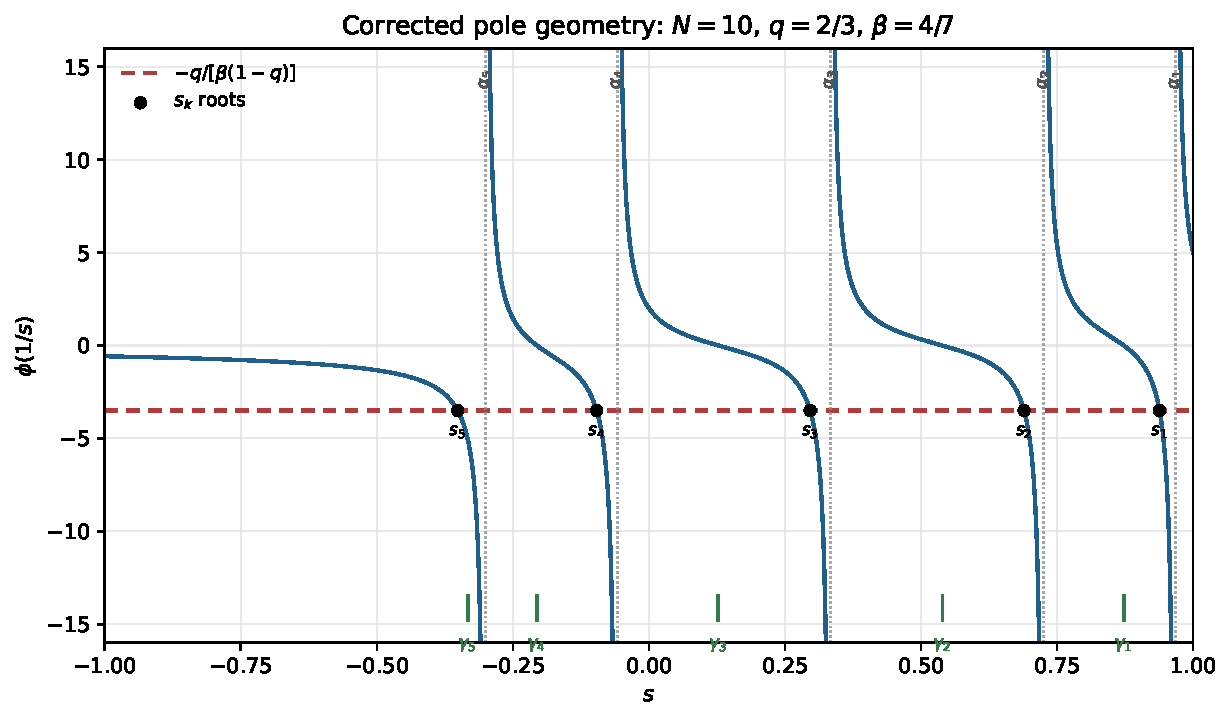
\includegraphics[width=0.92\linewidth]{phifunction.pdf}
\caption{Graphical representation of the poles of Eq. (\ref{eq:HNN2_}) for the case \(N=10\), \(q=2/3\), and \(\beta=4/7\).  The poles are the values of \(s\) where the horizontal line \(-q/[\beta(1-q)]\) intercepts \(\phi(1/s)\).  The asymptotes of \(\phi(1/s)\) are given by the \(\alpha_k\), and the paired tick marks indicate the corresponding \(\gamma_k\).  This figure is a visualization of the \(H\)-poles; the finite-time one-peak/two-peak transition is a property of the full first-passage distribution.}
\label{fig:phis}
\end{figure}
\FloatBarrier
It is useful to rewrite the same corrected \(H\) in a form tied directly to its denominator.  Let \(N=2L\),
\[
  a=\frac{q}{\beta(1-q)},\qquad y=1+\frac{1/z-1}{q}.
\]
Then
\begin{align}
\widetilde H_{N,N/2}(z)=
\frac{T_L(y)}{aT_L(y)+U_{L-1}(y)}.
\label{eq:H_closed}
\end{align}
If \(D(y)=aT_L(y)+U_{L-1}(y)\), \(D(y_k)=0\), and \(s_k=1-q+qy_k\), then the positive-time part of \(H\) can be written, for simple roots, as
\begin{align}
 H_{N,N/2}(t)=\sum_k c_k\,s_k^{t-1},\qquad
 c_k=\frac{qT_L(y_k)}{D'(y_k)},\qquad t\geq 1.
\label{eq:inv_z_t}
\end{align}
This residue form keeps the \(H(0)=\beta(1-q)/q\) contribution separate from the positive-time pole expansion.

The time dependence of Eq. (\ref{eq:first_pass_prob_2}) for $|u-v|=N/2$ is therefore given by the time-convoluted expression for $t\geq 1$
\begin{align}
F_{n_0}(v,t)=\mathcal{F}_{n_0}(v,t)+q\sum_{t^{\prime}=0}^{t-1}W_{n_0}(u,t-1-t^{\prime})\sum_{t^{\prime\prime}=0}^{t^{\prime}}\left[\delta_{t^{\prime},t^{\prime\prime}}-\mathcal{F}_{u}(v,t^{\prime}-t^{\prime\prime})\right]H_{N,N/2}(t^{\prime\prime})
\label{eq:fp_time}
\end{align}
and $F_{n_0}(v,0)=0$.

The same result can be written more compactly at the generating-function level.  Let \(\rho\) denote the folded distance of the starting site from the absorbing target in the antipodal case.  Using
\begin{align}
  \widetilde{\mathcal F}_{\rho}(0,z)&=\frac{T_{L-\rho}(y)}{T_L(y)},\\
  \widetilde W_{\rho}(L,z)&=\frac{U_{\rho-1}(y)}{zq\,T_L(y)},\\
  1-\widetilde{\mathcal F}_{L}(0,z)&=\frac{T_L(y)-1}{T_L(y)},\\
  \widetilde H_{N,N/2}(z)&=\frac{T_L(y)}{aT_L(y)+U_{L-1}(y)},
\end{align}
Eq. (\ref{eq:first_pass_prob_2}) reduces to
\begin{align}
\widetilde F_{\rho}(0,z)
&=
\frac{T_{L-\rho}(y)}{T_L(y)}
+\frac{U_{\rho-1}(y)\bigl[T_L(y)-1\bigr]}
{T_L(y)\bigl[aT_L(y)+U_{L-1}(y)\bigr]} \nonumber\\
&=
\frac{aT_{L-\rho}(y)+U_{\rho-1}(y)+U_{L-\rho-1}(y)}
{aT_L(y)+U_{L-1}(y)}.
\label{eq:corrected_closed_F}
\end{align}
The second equality uses
\[
  T_L(y)U_{L-\rho-1}(y)=T_{L-\rho}(y)U_{L-1}(y)-U_{\rho-1}(y).
\]
Here and below \(U_{-1}(y)=0\), which covers the endpoint case \(\rho=L\).
This cancellation should be read as a cancellation in the fully collected rational function, not as an attempt to determine poles from a numerator alone.  Before reduction, Eq. (\ref{eq:corrected_closed_F}) has the common denominator \(T_L(y)\{aT_L(y)+U_{L-1}(y)\}\), so the zeros of \(T_L(y)\) are candidate poles at that unreduced stage.  The numerator over this common denominator is
\[
  M_\rho(y)=T_{L-\rho}(y)\{aT_L(y)+U_{L-1}(y)\}
  +U_{\rho-1}(y)\{T_L(y)-1\}.
\]
This \(M_\rho(y)\) is a polynomial expression in \(y\), with no hidden \(1/T_L(y)\) factor.  The Chebyshev identity above then gives
\[
  M_\rho(y)=T_L(y)\left[aT_{L-\rho}(y)+U_{\rho-1}(y)+U_{L-\rho-1}(y)\right].
\]
Thus \(T_L(y)\) is a common analytic factor of the collected numerator and denominator.  It can be removed only after this collection step.  The expanded-route check in the Appendix shows the same cancellation explicitly, including the diagonal limits in the time-domain partial fractions.

The tail implication is therefore best read from the collected expression, not from the uncollected term-by-term convolution.  The apparent \(\alpha_\ell\)-modes that arise in the time-domain hard route correspond to the zeros of \(T_L(y)\).  They are removable singularities of the collected expression after the common \(T_L(y)\) factor is removed.  Hence the long-time behaviour is determined by the zeros of
\[
  D(y)=aT_L(y)+U_{L-1}(y).
\]
It is not determined by the zeros of \(T_L(y)\).  If \(D(y_k)=0\) and \(s_k=1-q+qy_k\), then for simple roots
\begin{align}
F_\rho(0,t)=\sum_k B_{\rho k}s_k^{t-1},\qquad
B_{\rho k}=\frac{q\left[aT_{L-\rho}(y_k)+U_{\rho-1}(y_k)+U_{L-\rho-1}(y_k)\right]}{D'(y_k)}.
\label{eq:tail_residue}
\end{align}
Therefore, ordering the roots so that \(s_1\) is the dominant positive pole, the corrected long-time dependence is
\[
  F_\rho(0,t)\sim B_{\rho 1}s_1^{t-1},\qquad t\to\infty.
\]
The dominant amplitude is not merely assumed nonzero: \(B_{\rho 1}>0\) strictly for every \(\rho,q,\beta\), proved in Appendix C from the compact form Eq. (\ref{eq:app_B1_positive}) and verified there to \(50\) digits.
Equivalently, the exponential decay rate is \(-\log s_1\).  The dependence on the shortcut strength enters through
\[
  a=\frac{q}{\beta(1-q)}
\]
in the denominator \(D(y)=aT_L(y)+U_{L-1}(y)\), and hence through the movement of the dominant root \(s_1=1-q+qy_1\).  Thus the corrected shortcut calculation changes the tail by moving the dominant pole; it does not produce a generic \(t\alpha_1^t\) long-time correction.

Two structural facts make the absence of the \(t\alpha_\ell^t\) factor exact rather than accidental.
First, the apparent double pole of the product \(\widetilde W_{n_0}(u,z)\bigl[1-\widetilde{\mathcal F}_u(v,z)\bigr]\) at \(z=1/\alpha_\ell\) is always accompanied by a \emph{zero} of \(\widetilde H\) at exactly the same point.  From Eq. (\ref{eq:HNuv}),
\begin{align}
\widetilde H_{N,N/2}(z)=\frac{\beta(1-q)}{q}\,
\frac{1}{1+z\beta(1-q)\widetilde W_u(u,z)}
\;\longrightarrow\;0
\qquad (z\to1/\alpha_\ell),
\label{eq:H_zero_at_alpha}
\end{align}
because the same killed propagator \(\widetilde W_u(u,z)\) that supplies the \(\alpha_\ell\)-modes of the numerator factors diverges in the denominator of \(\widetilde H\).  Every \(\alpha_\ell\) is a pole of \(\widetilde W_u(u,z)\) with residue coefficient \(g^{(2)}_\ell(u,u,v)=2/N\neq0\), so \(\widetilde H(1/\alpha_\ell)=0\) for every \(\ell=1,\ldots,L\) and every \(\beta>0\).  The would-be double pole is thereby reduced to at most a simple pole, and the residual simple-pole part cancels against the baseline \(\widetilde{\mathcal F}_{n_0}(v,z)\) through the residue identity
\[
  f_\ell(n_0,v)\,g^{(2)}_\ell(u,u,v)=g^{(2)}_\ell(n_0,u,v)\,f_\ell(u,v),
\]
which holds term by term from the definitions in Eqs. (\ref{eq:fn0m}) and (\ref{eq:small_g}).  This is the same statement as the \(T_L(y)\) factorization above.  Appendix A.4 shows the corresponding cancellation directly in the time domain: the total coefficient of the diagonal secular term \((t-1)\alpha_\ell^{t-2}\) is proportional to \(\sum_j c_j/(s_j-\alpha_\ell)-\beta(1-q)/q\), and this bracket vanishes identically by the sum rule in Eq. (\ref{eq:app_sum_rule}), which is nothing but \(\widetilde H(1/\alpha_\ell)=0\).  So the disappearance of the \(t\alpha_\ell^t\) coefficient is not a fine-tuned coincidence: it is forced, for every \(\ell\) and every admissible \((N,q,\beta)\), by the structure of \(\widetilde H\).

Second, no parameter choice can make a \(t\lambda^t\) term survive in this model at all.  For \(t\geq1\) the first-passage probability is a linear functional of powers of the transient submatrix of the shortcut chain (all rows and columns except the absorbing site \(v\)).  That submatrix is a \emph{symmetric tridiagonal (Jacobi) matrix with positive off-diagonal entries}: deleting \(v\) turns the ring into a path with off-diagonal entries \(q/2\) and diagonal \(1-q\), and the directed shortcut only lowers the diagonal entry at \(u\) to \(1-q-\beta(1-q)\), because the reallocated mass \(\beta(1-q)\) leaves through the absorbing column.  A Jacobi matrix with positive off-diagonals is diagonalizable with real and \emph{simple} spectrum for every parameter choice, so the exact PMF is a pure sum of geometric modes \(\sum_i\kappa_i\lambda_i^t\); a secular term \(t\lambda^t\) would require a defective (Jordan-block) eigenvalue, which such a matrix cannot have, and even accidental eigenvalue degeneracies are excluded.  The reflection symmetry \(n\mapsto N-n\) splits the eigenvectors into \(L-1\) antisymmetric modes, which vanish at \(u\) and keep the unperturbed eigenvalues \(\gamma_r\), and \(L\) symmetric modes, whose eigenvalues are exactly the roots \(s_j\) of \(D(y)\), strictly interlacing the \(\alpha_\ell\) for every \(\beta>0\).  Hence for \(\beta>0\) the values \(\alpha_\ell\) are not in the spectrum, since \(D(\eta_\ell)=U_{L-1}(\eta_\ell)\neq0\), and a \(t\alpha_\ell^t\) contribution is impossible rather than merely cancelled; likewise \(s_j=\gamma_r\) never occurs, since \(D=a(-1)^r\neq0\) at every \(\gamma_r\) location (Appendix C).  Finally, the one-step absorption vector is reflection symmetric, so the antisymmetric \(\gamma_r\)-modes carry zero amplitude in the first-passage probability for \emph{every} starting site; this is why Eq. (\ref{eq:tail_residue}) contains only the \(s_j\), in agreement with the explicit \(G^{(1)}_r=0\) computation noted after Eq. (\ref{eq:app_W_modes}).

The finite-time one-peak/two-peak transition is therefore a shape question for the full first-passage distribution, not a criterion obtained from the auxiliary \(H\)-pole plot alone.  In particular, the proposed crossing \(s_1=\gamma_1=1-q+q\cos(2\pi/N)\) does not occur for any finite positive \(\beta\); the dominant corrected pole satisfies \(\gamma_1<s_1<\alpha_1\) for all \(0<q<1\) and \(0<\beta\leq1\), by the sign argument in Appendix C (\(D=-a<0\) at the \(\gamma_1\) location, \(D=U_{L-1}(\eta_1)>0\) at the \(\alpha_1\) location, and \(D>0\) above it).
The deterministic finite-matrix numerical audit used to check these statements is recorded in Appendix C, including the direct shortcut matrix benchmark and the five-group check of Eq. (\ref{eq:app_hard_route_result}).

\clearpage
\appendix
\section*{Appendix A: Direct time-domain route}

This appendix carries out the corrected calculation in the same time-convolution route as the long displayed expansion.  The goal is to make clear which terms arise before simplification, and why the collected answer is the compact closed form in Eq. (\ref{eq:corrected_closed_F}).  Throughout this appendix
\[
  N=2L,\qquad L\geq 2,\qquad 0<q<1,\qquad 0<\beta\leq 1,
\]
the absorbing target is \(v=0\), the shortcut source is \(u=L\), and \(1\leq \rho\leq L\) is the folded distance from the initial site to \(v\).  We also use
\[
  a=\frac{q}{\beta(1-q)},\qquad
  y=1+\frac{1/z-1}{q},\qquad
  U_{-1}(y)=0.
\]

\subsection*{A.1 Corrected convolution}

The corrected generating-function starting point is Eq. (\ref{eq:first_pass_prob_2}),
\begin{align}
\widetilde F_{n_0}(v,z)
&=\widetilde{\mathcal F}_{n_0}(v,z)
+qz\,\widetilde W_{n_0}(u,z)
\left[1-\widetilde{\mathcal F}_{u}(v,z)\right]\widetilde H_{N,N/2}(z).
\label{eq:app_time_route_gf}
\end{align}
Equivalently, for \(t\geq1\),
\begin{align}
F_{n_0}(v,t)
&=\mathcal F_{n_0}(v,t)
+q\sum_{t'=0}^{t-1}W_{n_0}(u,t-1-t')
\sum_{t''=0}^{t'}
\left[\delta_{t',t''}-\mathcal F_u(v,t'-t'')\right]H_{N,N/2}(t'').
\label{eq:app_time_route_conv}
\end{align}
This is the route expanded below.

\subsection*{A.2 Mode inputs}

For \(N=2L\), the no-shortcut first-passage probability is
\begin{align}
\mathcal F_{n_0}(v,t)
&=\sum_{\ell=1}^{L}f_\ell(n_0,v)\alpha_\ell^{t-1},\qquad t\geq1,
\label{eq:app_F0_modes}
\end{align}
where \(f_\ell\) is defined in Eq. (\ref{eq:fn0m}) with the odd index \(2\ell-1\), and
\[
  \alpha_\ell=1-q+q\cos\frac{(2\ell-1)\pi}{N}.
\]
From Eq. (\ref{eq:compactprob_abs}), evaluated at the shortcut source \(u\), we write
\begin{align}
W_{n_0}(u,t)
&=\sum_{r=1}^{N-1}G^{(1)}_r(n_0,u,v)\gamma_r^t
+\sum_{r=1}^{L}g^{(2)}_r(n_0,u,v)\alpha_r^t,
\label{eq:app_W_modes}
\end{align}
where
\[
  \gamma_r=1-q+q\cos\frac{2\pi r}{N},
  \qquad
  g^{(2)}_r(n_0,u,v)=G^{(2)}_{2r-1}(n_0,u,v).
\]
The even \(G^{(2)}\)-terms vanish because of the factor \(1-(-1)^k\).
In the antipodal geometry the \(G^{(1)}\)-coefficients of Eq. (\ref{eq:app_W_modes}) vanish identically as well: with \(u-v=N/2\),
\(\cos[2\pi r(u-n_0)/N]=(-1)^r\cos[2\pi r(n_0-v)/N]\) and \(\cos[2\pi r(u-v)/N]=(-1)^r\), so \(G^{(1)}_r(n_0,u,v)=0\) for every \(r\).  The killed propagator evaluated at the antipodal point is therefore a pure \(\alpha\)-mode sum, consistent with the closed form \(\widetilde W_\rho(L,z)=U_{\rho-1}(y)/[zq\,T_L(y)]\), whose denominator contains no \(U_{L-1}(y)\) factor.  The \(G^{(1)}\)-pieces are nevertheless kept in the displays below so that the term-by-term correspondence with the previous long Eq.~(41)-style expression remains visible; in the antipodal case they contribute zero.

For the antipodal shortcut,
\begin{align}
\widetilde H_{N,N/2}(z)
&=\frac{T_L(y)}{D(y)},\qquad
D(y)=aT_L(y)+U_{L-1}(y).
\label{eq:app_H_D}
\end{align}
The \(H(0)\) term must be kept separate:
\[
  h_0=H_{N,N/2}(0)=\frac{\beta(1-q)}{q}=\frac{1}{a}.
\]
If \(D(y_j)=0\) and \(s_j=1-q+qy_j\), then the positive-time part is
\begin{align}
H_{N,N/2}(t)
&=\sum_j c_j s_j^{t-1},\qquad
c_j=\frac{qT_L(y_j)}{D'(y_j)},\qquad t\geq1.
\label{eq:app_H_residue}
\end{align}

\subsection*{A.3 Convolution kernels}

The \(\delta\)-term in Eq. (\ref{eq:app_time_route_conv}) gives a two-factor convolution.  The \(H(0)\) part is simply
\[
  A^{(0)}_t(x)=x^{t-1}.
\]
For a positive-time \(H\)-pole,
\begin{align}
A^{(+)}_t(x;s)
&=\sum_{c=1}^{t-1}x^{t-1-c}s^{c-1}
=\frac{s^{t-1}-x^{t-1}}{s-x}.
\label{eq:app_A_plus}
\end{align}
The coincident case \(x=s\) is understood as the limit
\[
  A^{(+)}_t(s;s)=(t-1)s^{t-2}.
\]

The negative \(\mathcal F_u(v,\cdot)\)-part gives a three-factor convolution.  With \(b\geq1\), the \(H(0)\) contribution is
\begin{align}
B^{(0)}_t(x,y)
&=\sum_{\substack{a+b=t-1\\ b\geq1}}x^a y^{b-1}
=\frac{x^{t-1}-y^{t-1}}{x-y}.
\label{eq:app_B_zero}
\end{align}
The positive-time \(H\)-pole contribution is
\begin{align}
B^{(+)}_t(x,y;s)
&=\sum_{\substack{a+b+c=t-1\\ b\geq1,\ c\geq1}}x^a y^{b-1}s^{c-1}
\nonumber\\
&=\operatorname{Coeff}_{\xi^{t-3}}
\frac{1}{(1-\xi x)(1-\xi y)(1-\xi s)}.
\label{eq:app_B_plus_def}
\end{align}
When \(x,y,s\) are distinct,
\begin{align}
B^{(+)}_t(x,y;s)
&=
\frac{x^{t-1}}{(x-y)(x-s)}
+\frac{y^{t-1}}{(y-x)(y-s)}
+\frac{s^{t-1}}{(s-x)(s-y)}.
\label{eq:app_B_plus_distinct}
\end{align}
Coincident cases are obtained by taking limits.  This is the point at which an uncollected term-by-term expansion can temporarily produce factors such as \(t\alpha_\ell^t\); those factors are not tail terms unless they survive after the complete expression is recombined.

\subsection*{A.4 Corrected Eq. (41)-style expansion}

Substituting Eqs. (\ref{eq:app_F0_modes}), (\ref{eq:app_W_modes}), and (\ref{eq:app_H_residue}) into Eq. (\ref{eq:app_time_route_conv}) gives the corrected long expansion.  To keep the direct comparison with the previous long Eq. (41)-style calculation transparent, all five convolution groups are written out below; no \(A_t\)- or \(B_t\)-kernel shorthand is used in the displayed result.
\begingroup
\scriptsize
\setlength{\jot}{3pt}
\begin{align}
F_{n_0}(v,t)
&=
\sum_{\ell=1}^{L}f_\ell(n_0,v)\alpha_\ell^{t-1}
\nonumber\\
&\quad
+q h_0
\left[
\sum_{r=1}^{N-1}G^{(1)}_r(n_0,u,v)\gamma_r^{t-1}
+\sum_{r=1}^{L}g^{(2)}_r(n_0,u,v)\alpha_r^{t-1}
\right]
\nonumber\\
&\quad
+q\sum_j c_j
\left[
\sum_{r=1}^{N-1}G^{(1)}_r(n_0,u,v)
\frac{s_j^{t-1}-\gamma_r^{t-1}}{s_j-\gamma_r}
+\sum_{r=1}^{L}g^{(2)}_r(n_0,u,v)
\frac{s_j^{t-1}-\alpha_r^{t-1}}{s_j-\alpha_r}
\right]
\nonumber\\
&\quad
-q h_0\sum_{\ell=1}^{L}f_\ell(u,v)
\left[
\sum_{r=1}^{N-1}G^{(1)}_r(n_0,u,v)
\frac{\gamma_r^{t-1}-\alpha_\ell^{t-1}}{\gamma_r-\alpha_\ell}
\right.
\nonumber\\
&\hspace{35mm}\left.
+\sum_{\substack{r=1\\r\neq\ell}}^{L}g^{(2)}_r(n_0,u,v)
\frac{\alpha_r^{t-1}-\alpha_\ell^{t-1}}{\alpha_r-\alpha_\ell}
+g^{(2)}_\ell(n_0,u,v)(t-1)\alpha_\ell^{t-2}
\right]
\nonumber\\
&\quad
-q\sum_j c_j\sum_{\ell=1}^{L}f_\ell(u,v)
\left[
\sum_{r=1}^{N-1}G^{(1)}_r(n_0,u,v)
\left(
\frac{\gamma_r^{t-1}}{(\gamma_r-\alpha_\ell)(\gamma_r-s_j)}
+\frac{\alpha_\ell^{t-1}}{(\alpha_\ell-\gamma_r)(\alpha_\ell-s_j)}
+\frac{s_j^{t-1}}{(s_j-\gamma_r)(s_j-\alpha_\ell)}
\right)
\right.
\nonumber\\
&\hspace{35mm}\left.
+\sum_{\substack{r=1\\r\neq\ell}}^{L}g^{(2)}_r(n_0,u,v)
\left(
\frac{\alpha_r^{t-1}}{(\alpha_r-\alpha_\ell)(\alpha_r-s_j)}
+\frac{\alpha_\ell^{t-1}}{(\alpha_\ell-\alpha_r)(\alpha_\ell-s_j)}
+\frac{s_j^{t-1}}{(s_j-\alpha_r)(s_j-\alpha_\ell)}
\right)
\right.
\nonumber\\
&\hspace{35mm}\left.
+g^{(2)}_\ell(n_0,u,v)
\left(
\frac{s_j^{t-1}-\alpha_\ell^{t-1}}{(s_j-\alpha_\ell)^2}
-\frac{(t-1)\alpha_\ell^{t-2}}{s_j-\alpha_\ell}
\right)
\right].
\label{eq:app_hard_route_result}
\end{align}
\endgroup
Equation (\ref{eq:app_hard_route_result}) is the corrected direct-route replacement for the long Eq. (41)-style expression.  The baseline first-passage term targets \(v\), the global sign follows the positive sign in Eq. (\ref{eq:app_time_route_gf}), and the \(g^{(2)}\)-modes are paired with \(\alpha_r\).  The final term in the last bracket is the \(r=\ell\) diagonal limit of the \((\alpha_r,\alpha_\ell,s_j)\) triple convolution.  Thus the fully expanded hard-route form really does contain explicit \(\alpha_\ell\)-powers and \(t\alpha_\ell\)-type factors.  The point of the later recombination is not that these intermediate terms are absent, but that their apparent \(T_L(y)=0\) poles cancel after all five convolution groups are collected.

\medskip
\noindent\textbf{How Eq. (\ref{eq:app_hard_route_result}) is generated, and where the cancellation occurs.}
The correspondence with the previous long Eq. (41)-style expression is term-by-term, but not by a mere change of notation.  The first term of the previous long expression corresponds to the first line of Eq. (\ref{eq:app_hard_route_result}); the target in the baseline term is \(v\), so the coefficient is \(f_\ell(n_0,v)\), not \(f_\ell(n_0,u)\).  The first large \(s\)-dependent brace in the previous long expression corresponds to the second and third lines of Eq. (\ref{eq:app_hard_route_result}): the \(H(0)=h_0\) contribution has to be split off, giving the \(q h_0 W\) term, and only the positive-time part of \(H\) gives the difference quotients \((s_j^{t-1}-x^{t-1})/(s_j-x)\).  The previous \(G^{(1)}f_\ell(u,v)\) terms correspond to the \(G^{(1)}\)-parts in the fourth and fifth lines, written as a two-mode difference quotient and a three-mode partial fraction.  The previous \(g^{(2)}f_\ell(u,v)\) terms correspond to the \(g^{(2)}\)-parts in the fourth and fifth lines; here \(g^{(2)}_r\) is paired with the \(\alpha_r\)-mode.  Any visible \(t\alpha_\ell^t\) term is a coincident-limit case of the written-out partial fractions, not a final tail term.

The six term-level correspondences are the following.  To keep the displays readable, only in this paragraph write
\[
  G_r=G^{(1)}_r(n_0,u,v),\qquad
  g_r=g^{(2)}_r(n_0,u,v),\qquad
  f_\ell^{uv}=f_\ell(u,v),
  \qquad L=N/2.
\]

\begin{enumerate}
\item The no-shortcut baseline term is
\begin{align*}
\text{previous piece:}\qquad
&\sum_{\ell=1}^{L}f_\ell(n_0,u)\alpha_\ell^{t-1},\\
\text{corrected piece:}\qquad
&\sum_{\ell=1}^{L}f_\ell(n_0,v)\alpha_\ell^{t-1}.
\end{align*}
This is the first line of Eq. (\ref{eq:app_hard_route_result}); the target of the no-shortcut first passage is \(v\).

\item The first large \(s\)-dependent \(W\)-brace is replaced by the two pieces \(qW*\delta*h_0\delta_0\) and \(qW*\delta*H_+\):
\begin{align*}
\text{previous piece:}\qquad
&-q\sum_{k=1}^{M}\Bigg[
\sum_{r=1}^{N-1}
\frac{c_kG_r}{s_k(s_k-\gamma_r)}
\left(s_k^t-\gamma_r^t\right)
\nonumber\\[-1mm]
&\hspace{34mm}
+\sum_{\ell=1}^{L}
\frac{c_kg_\ell}{s_k(s_k-\alpha_\ell)}
\left(s_k^t-\alpha_\ell^t\right)
\Bigg],
\nonumber\\
\text{corrected pieces:}\qquad
&q h_0
\left[
\sum_{r=1}^{N-1}G_r\gamma_r^{t-1}
+\sum_{r=1}^{L}g_r\alpha_r^{t-1}
\right]
\nonumber\\
&\quad
+q\sum_j c_j
\left[
\sum_{r=1}^{N-1}G_r
\frac{s_j^{t-1}-\gamma_r^{t-1}}{s_j-\gamma_r}
+\sum_{r=1}^{L}g_r
\frac{s_j^{t-1}-\alpha_r^{t-1}}{s_j-\alpha_r}
\right].
\end{align*}
These are the second and third lines of Eq. (\ref{eq:app_hard_route_result}).  The sign changes because the corrected route uses \(+qW*(\delta-\mathcal F_u)*H\), and \(H(0)=h_0\) is no longer folded into the positive-time pole expansion.

\item The power shift in the old \(s\)-dependent factors is exactly the \(H(0)\) separation:
\begin{align*}
\text{old kernel if the positive-time pole is used at time zero:}\qquad
&\sum_{c=0}^{t-1}x^{t-1-c}s^{c-1}
=\frac{s^t-x^t}{s(s-x)},\\
\text{corrected positive-time sum:}\qquad
&\sum_{c=1}^{t-1}x^{t-1-c}s^{c-1}
=\frac{s^{t-1}-x^{t-1}}{s-x}.
\end{align*}
This is why the corrected Eq. (\ref{eq:app_hard_route_result}) uses the \((s^{t-1}-x^{t-1})/(s-x)\) difference quotient rather than the old-looking \((s^t-x^t)/(s(s-x))\) factors.

\item The \(G^{(1)}f_\ell(u,v)\) triple-convolution terms are
\begin{align*}
\text{previous piece:}\qquad
&q\sum_{k=1}^{M}\sum_{r=1}^{N-1}\sum_{\ell=1}^{L}
\frac{c_kG_rf_\ell^{uv}}{s_k-\alpha_\ell}
\left[
\frac{s_k^t-\gamma_r^t}{\alpha_\ell(s_k-\gamma_r)}
-\frac{\alpha_\ell^t-\gamma_r^t}{s_k(\alpha_\ell-\gamma_r)}
\right],
\nonumber\\
\text{corrected pieces:}\qquad
&-q h_0\sum_{\ell=1}^{L}f_\ell^{uv}
\sum_{r=1}^{N-1}G_r
\frac{\gamma_r^{t-1}-\alpha_\ell^{t-1}}{\gamma_r-\alpha_\ell}
\nonumber\\
&\quad
-q\sum_j c_j\sum_{\ell=1}^{L}f_\ell^{uv}
\sum_{r=1}^{N-1}G_r
\left(
\frac{\gamma_r^{t-1}}{(\gamma_r-\alpha_\ell)(\gamma_r-s_j)}
\right.
\nonumber\\[-1mm]
&\hspace{18mm}\left.
+\frac{\alpha_\ell^{t-1}}{(\alpha_\ell-\gamma_r)(\alpha_\ell-s_j)}
+\frac{s_j^{t-1}}{(s_j-\gamma_r)(s_j-\alpha_\ell)}
\right).
\end{align*}
These are the \(G^{(1)}\)-parts of the fourth and fifth lines of Eq. (\ref{eq:app_hard_route_result}).

\item The off-diagonal \(g^{(2)}f_\ell(u,v)\) terms are
\begin{align*}
\text{previous piece:}\qquad
&q\sum_{k=1}^{M}
\sum_{\substack{r,\ell=1\\ r\neq\ell}}^{L}
\frac{c_kg_rf_\ell^{uv}}{s_k\alpha_\ell(s_k-\alpha_\ell)}
\left[
s_k\frac{s_k^t-\gamma_r^t}{s_k-\gamma_r}
-\alpha_\ell\frac{\alpha_\ell^t-\gamma_r^t}{\alpha_\ell-\gamma_r}
\right],
\nonumber\\
\text{corrected pieces:}\qquad
&-q h_0\sum_{\ell=1}^{L}f_\ell^{uv}
\sum_{\substack{r=1\\ r\neq\ell}}^{L}
g_r
\frac{\alpha_r^{t-1}-\alpha_\ell^{t-1}}{\alpha_r-\alpha_\ell}
\nonumber\\
&\quad
-q\sum_j c_j\sum_{\ell=1}^{L}f_\ell^{uv}
\sum_{\substack{r=1\\ r\neq\ell}}^{L}
g_r
\left(
\frac{\alpha_r^{t-1}}{(\alpha_r-\alpha_\ell)(\alpha_r-s_j)}
\right.
\nonumber\\[-1mm]
&\hspace{18mm}\left.
+\frac{\alpha_\ell^{t-1}}{(\alpha_\ell-\alpha_r)(\alpha_\ell-s_j)}
+\frac{s_j^{t-1}}{(s_j-\alpha_r)(s_j-\alpha_\ell)}
\right).
\end{align*}
The corrected \(g_r\)-mode is paired with \(\alpha_r\), not with \(\gamma_r\).

\item The visible diagonal \(t\alpha_\ell^t\) term is the \(r=\ell\) coincident-limit case of the same corrected kernels:
\begin{align*}
\text{previous diagonal piece:}\qquad
&-q\sum_{k=1}^{M}\sum_{\ell=1}^{L}
\frac{c_kg_\ell f_\ell^{uv}}{s_k\alpha_\ell(s_k-\alpha_\ell)}
\alpha_\ell^t\,t,
\nonumber\\
\text{corrected diagonal pieces:}\qquad
&-q h_0\sum_{\ell=1}^{L}
f_\ell^{uv}g_\ell(t-1)\alpha_\ell^{t-2}
\nonumber\\
&\quad
-q\sum_j c_j\sum_{\ell=1}^{L}
f_\ell^{uv}g_\ell
\left[
\frac{s_j^{t-1}-\alpha_\ell^{t-1}}{(s_j-\alpha_\ell)^2}
-\frac{(t-1)\alpha_\ell^{t-2}}{s_j-\alpha_\ell}
\right],
\end{align*}
where the square bracket is the same as
\[
  \sum_{c=1}^{t-2}(t-1-c)\alpha_\ell^{t-2-c}s_j^{c-1}.
\]
Thus the \(t\alpha_\ell^t\)-type factor is only a diagonal-limit term in the uncollected expansion.  It is not a final tail term unless the corresponding \(\alpha_\ell\)-pole survives the complete recombination, which it does not.
\end{enumerate}

Thus the long Eq. (\ref{eq:app_hard_route_result}) is obtained by following the term-by-term route and keeping the partial fractions separated.  Write
\[
  H(t)=h_0\delta_{t,0}+H_+(t),
  \qquad
  H_+(t)=\sum_j c_j s_j^{t-1}\quad (t\geq1).
\]
Then the five groups in Eq. (\ref{eq:app_hard_route_result}) come from the five pieces
\[
\begin{array}{rcl}
\mathcal F_{n_0}(v,\cdot) &\longrightarrow& \text{first line of Eq. (\ref{eq:app_hard_route_result})},\\
q\,W_{n_0}(u,\cdot)*\delta* h_0\delta_0
&\longrightarrow& \text{second line},\\
q\,W_{n_0}(u,\cdot)*\delta*H_+
&\longrightarrow& \text{third line},\\
-q\,W_{n_0}(u,\cdot)*\mathcal F_u(v,\cdot)*h_0\delta_0
&\longrightarrow& \text{fourth line},\\
-q\,W_{n_0}(u,\cdot)*\mathcal F_u(v,\cdot)*H_+
&\longrightarrow& \text{fifth line}.
\end{array}
\]
The sign pattern comes directly from the corrected shortcut contribution \(+q\,W*(\delta-\mathcal F_u)*H\): the two \(\delta\)-pieces are positive, and the two \(\mathcal F_u\)-pieces are negative.
This is the same mechanical route that produces a long Eq. (41)-style expression: insert the modal forms for \(\mathcal F\), \(W\), and \(H\), do the finite time sums, and leave the answer as separated partial fractions.  At that stage the \(\alpha_\ell\)-dependent pieces are visible because the no-shortcut first-passage and killed-propagator modes contain \(\alpha_\ell\).  Reading the tail directly from this uncollected list is premature.

The cancellation is not a cancellation inside a single displayed line of Eq. (\ref{eq:app_hard_route_result}).  It occurs when all five groups are recombined before the pole set is read.  In generating-function form those same five groups add to
\[
\frac{T_{L-\rho}(y)}{T_L(y)}
+
\frac{U_{\rho-1}(y)\left[T_L(y)-1\right]}{T_L(y)D(y)}.
\]
Putting this over the common denominator \(T_L(y)D(y)\) gives Eq. (\ref{eq:app_expanded_common_denominator}).  The numerator is then
\[
  aT_{L-\rho}(y)T_L(y)+T_{L-\rho}(y)U_{L-1}(y)
  +U_{\rho-1}(y)T_L(y)-U_{\rho-1}(y),
\]
and the Chebyshev identity factors this numerator as
\[
  T_L(y)\left[aT_{L-\rho}(y)+U_{\rho-1}(y)+U_{L-\rho-1}(y)\right].
\]
This displayed \(T_L(y)\) factor cancels the apparent \(T_L(y)\) in the common denominator.  Therefore the \(\alpha_\ell\)-modes that appear while deriving Eq. (\ref{eq:app_hard_route_result}) are removable intermediate modes, not final tail poles.

\medskip
\noindent\textbf{Explicit vanishing of the diagonal secular coefficient.}
The cancellation of the \(t\alpha_\ell^t\)-type terms can also be checked by simple algebra directly in the time domain, without any generating-function collection.  In Eq. (\ref{eq:app_hard_route_result}) the only terms proportional to \((t-1)\alpha_\ell^{t-2}\) are the two diagonal pieces, one from the \(h_0\)-group (fourth line) and one from the \(H_+\)-group (fifth line):
\[
  -q\,h_0\,f_\ell(u,v)\,g^{(2)}_\ell(n_0,u,v)\,(t-1)\alpha_\ell^{t-2}
  \qquad\text{and}\qquad
  +q\,f_\ell(u,v)\,g^{(2)}_\ell(n_0,u,v)\,(t-1)\alpha_\ell^{t-2}\sum_j\frac{c_j}{s_j-\alpha_\ell}\,.
\]
Their sum carries the total secular coefficient
\begin{align}
  \mathcal K_\ell
  =q\,f_\ell(u,v)\,g^{(2)}_\ell(n_0,u,v)
  \left[\sum_j\frac{c_j}{s_j-\alpha_\ell}-h_0\right].
  \label{eq:app_secular_coeff}
\end{align}
The bracket vanishes identically because of the sum rule
\begin{align}
  \sum_j\frac{c_j}{s_j-\alpha_\ell}=h_0=\frac{\beta(1-q)}{q},
  \qquad \ell=1,\ldots,L,
  \label{eq:app_sum_rule}
\end{align}
so \(\mathcal K_\ell=0\) for every \(\ell\), every starting site, and every admissible \((N,q,\beta)\) with \(\beta>0\).  No special combination of parameters is needed.

The sum rule itself is three lines of partial fractions.  Write \(s=1/z\), so that \(y=1+(s-1)/q\) is affine in \(s\), and define \(\widehat H(s)=\widetilde H_{N,N/2}(1/s)\).  Since \(y-\eta_\ell=(s-\alpha_\ell)/q\) at the zeros \(\eta_\ell=\cos[(2\ell-1)\pi/(2L)]\) of \(T_L\), and \(y-\cos(r\pi/L)=(s-\gamma_r)/q\) at the zeros of \(U_{L-1}\),
\begin{align}
  T_L(y(s))=\frac{2^{L-1}}{q^{L}}\prod_{\ell=1}^{L}(s-\alpha_\ell),
  \qquad
  D(y(s))=\frac{2^{L-1}}{q^{L}}\,\Delta(s),
  \qquad
  \Delta(s)=a\prod_{j=1}^{L}(s-s_j),
  \label{eq:app_s_factorizations}
\end{align}
where the last equality holds because \(\Delta(s)=a\prod_\ell(s-\alpha_\ell)+q\prod_r(s-\gamma_r)\) is a degree-\(L\) polynomial with leading coefficient \(a\) whose roots are by definition the \(s_j\).  Hence
\begin{align}
  \widehat H(s)
  =\frac{\prod_{\ell=1}^{L}(s-\alpha_\ell)}{a\prod_{j=1}^{L}(s-s_j)}
  =\frac1a+\sum_j\frac{c_j}{s-s_j},
  \qquad
  c_j=\frac{\prod_{\ell}(s_j-\alpha_\ell)}{a\prod_{i\neq j}(s_j-s_i)},
  \label{eq:app_Hhat_pf}
\end{align}
which is the same partial-fraction data as \(c_j=qT_L(y_j)/D'(y_j)\), and the constant term \(1/a=h_0\) reproduces \(H(0)\).  Evaluating Eq. (\ref{eq:app_Hhat_pf}) at \(s=\alpha_m\) makes the left side vanish, because \(\alpha_m\) is a zero of the numerator \(\prod_\ell(s-\alpha_\ell)\):
\[
  0=\widehat H(\alpha_m)=h_0+\sum_j\frac{c_j}{\alpha_m-s_j}
  \qquad\Longleftrightarrow\qquad
  \sum_j\frac{c_j}{s_j-\alpha_m}=h_0 .
\]
This is Eq. (\ref{eq:app_sum_rule}); it is the time-domain face of the statement \(\widetilde H(1/\alpha_m)=0\) of Eq. (\ref{eq:H_zero_at_alpha}).  The zero is structural: the same \(\widetilde W_u(u,z)\) that supplies the \(\alpha_\ell\)-modes to \(W_{n_0}(u,\cdot)\) and \(\mathcal F_u(v,\cdot)\) sits in the denominator of \(\widetilde H\), so \(\widetilde H\) vanishes at every \(\alpha\)-location simultaneously.  The analogous evaluation at \(s=\gamma_r\), where \(U_{L-1}\) vanishes so that \(\Delta(\gamma_r)=a\prod_\ell(\gamma_r-\alpha_\ell)\) cancels the numerator of Eq. (\ref{eq:app_Hhat_pf}) exactly, gives \(\widehat H(\gamma_r)=1/a=h_0\) and hence \(\sum_jc_j/(\gamma_r-s_j)=0\): the \(\gamma\)-modes pass through the shortcut kernel with no net weight, consistent with their zero amplitude in the final tail expression.

\medskip
\noindent\textbf{The plain \(\alpha_\ell^{t-1}\) coefficients vanish as well.}
The same bookkeeping closes the time-domain argument completely: not only the secular diagonal, but every \(\alpha_\ell\)-dependent term of Eq. (\ref{eq:app_hard_route_result}) cancels explicitly, so no appeal to pole locations of any collected expression is needed.  Collect the coefficient of \(\alpha_\ell^{t-1}\) group by group (recall \(G^{(1)}_r=0\) in the antipodal geometry).
(i) \emph{\(W\)-mode terms} (second and third lines): the \(h_0\)-piece contributes \(+q h_0 g^{(2)}_\ell\), and the \(H_+\)-difference quotients contribute \(-q g^{(2)}_\ell\sum_jc_j/(s_j-\alpha_\ell)\); by the sum rule (\ref{eq:app_sum_rule}) these add to zero.
(ii) \emph{Off-diagonal \(\mathcal F_u\)-terms} (fourth and fifth lines, \(r\neq\ell\)): both carry the same bracket
\(X_\ell=g^{(2)}_\ell\sum_{m\neq\ell}f_m(u,v)/(\alpha_\ell-\alpha_m)+f_\ell(u,v)\sum_{m\neq\ell}g^{(2)}_m/(\alpha_\ell-\alpha_m)\),
the \(h_0\)-group with weight \(-qh_0\) and the \(H_+\)-group with weight \(-q\sum_jc_j/(\alpha_\ell-s_j)=+qh_0\); they cancel pairwise, again by the sum rule.
(iii) \emph{Diagonal remainder}: the surviving \(\alpha_\ell^{t-1}\) pieces are the baseline \(f_\ell(n_0,v)\) and the \(-\alpha_\ell^{t-1}/(s_j-\alpha_\ell)^2\) part of the diagonal kernel, giving the total
\begin{align}
  \Bigl[f_\ell(n_0,v)+q\,f_\ell(u,v)\,g^{(2)}_\ell(n_0,u,v)\sum_j\frac{c_j}{(s_j-\alpha_\ell)^2}\Bigr]\alpha_\ell^{t-1}.
  \label{eq:app_plain_alpha_total}
\end{align}
This vanishes by a second, derivative sum rule.  Differentiating Eq. (\ref{eq:app_Hhat_pf}) and evaluating at \(s=\alpha_m\), where \(T_L\) vanishes while \(D(\eta_m)=U_{L-1}(\eta_m)\) and \(T_L'(\eta_m)=L\,U_{L-1}(\eta_m)\),
\begin{align}
  \sum_j\frac{c_j}{(s_j-\alpha_m)^2}
  =-\widehat H'(\alpha_m)
  =-\frac{T_L'(\eta_m)}{q\,D(\eta_m)}
  =-\frac{L}{q},
  \qquad m=1,\ldots,L,
  \label{eq:app_derivative_sum_rule}
\end{align}
remarkably independent of \(\beta\).  Substituting into Eq. (\ref{eq:app_plain_alpha_total}) and using \(\sin^2[(2\ell-1)\pi L/N]=1\), the bracket becomes
\[
  f_\ell(n_0,v)-\frac{N}{2}\,f_\ell(u,v)\,g^{(2)}_\ell(n_0,u,v)
  =\frac{2q}{N}\sin\frac{(2\ell-1)\pi\rho}{N}\sin\frac{(2\ell-1)\pi}{N}
  -\frac{2q}{N}\sin\frac{(2\ell-1)\pi\rho}{N}\sin\frac{(2\ell-1)\pi}{N}=0 ,
\]
which is the residue identity quoted in the main text.  Hence \emph{every} \(\alpha_\ell\)-dependent term of Eq. (\ref{eq:app_hard_route_result}) --- \(W\)-mode, off-diagonal, diagonal-secular, and plain --- cancels explicitly in the time domain, and the only surviving modes are the \(s_j^{t-1}\), in agreement with the closed form Eq. (\ref{eq:app_tail_residue}).  Both sum rules, Eqs. (\ref{eq:app_sum_rule}) and (\ref{eq:app_derivative_sum_rule}), are verified to \(50\)-digit precision in Appendix C.1.1.

\medskip
\noindent\textbf{Where a spurious \(t\alpha_\ell^t\) term comes from.}
The previous long Eq.~(41)-style route used kernels of the form
\[
  \frac{s_j^{t}-x^{t}}{s_j(s_j-x)}=\sum_{c=0}^{t-1}x^{t-1-c}s_j^{c-1},
\]
that is, it extended the positive-time pole expansion \(H(t'')=\sum_j c_js_j^{t''-1}\) down to \(t''=0\).  This silently replaces the true \(H(0)=h_0\) by
\[
  \sum_j\frac{c_j}{s_j}=h_0-c_\infty,
  \qquad
  c_\infty=\widehat H(0)=\frac{T_L(1-1/q)}{D(1-1/q)}\neq0,
\]
where the expression for \(c_\infty\) follows from Eq. (\ref{eq:app_Hhat_pf}) at \(s=0\), i.e.\ from \(y(0)=1-1/q\).  Carrying the same diagonal collection with \(h_0\) replaced by \(h_0-c_\infty\) turns the bracket in Eq. (\ref{eq:app_secular_coeff}) into \(+c_\infty\), so the diagonal secular term acquires the nonzero coefficient
\[
  \mathcal K^{\mathrm{folded}}_\ell=q\,f_\ell(u,v)\,g^{(2)}_\ell(n_0,u,v)\,c_\infty
\]
instead of zero.  This is precisely the origin of the apparent ``logarithmic correction'': it measures the time-zero boundary mismatch of the \(H\)-pole expansion, not a property of the first-passage tail.  For \(N=10\), \(q=2/3\), \(\beta=4/7\) one finds \(c_\infty=2/11\) exactly, and the folded-kernel route deviates from the exact finite-matrix PMF by \(q f_1(u,v)g^{(2)}_1 c_\infty\,(t-1)\alpha_1^{t-2}\,[1+o(1)]\), while the exact-\(H(0)\) route of Eq. (\ref{eq:app_hard_route_result}) agrees with the finite matrix to better than \(10^{-51}\) in 50-digit arithmetic; see Appendix C.

\subsection*{\texorpdfstring{A.5 Generating-function recombination of Eq. (\ref{eq:app_hard_route_result})}{A.5 Generating-function recombination of the expanded route}}

One can also see directly that Eq. (\ref{eq:app_hard_route_result}) recombines into the generating-function route used below.  Use the transform
\[
  \mathcal Z[X_t](z)=\sum_{t\geq1}X_tz^t.
\]
The convolution kernels in Appendix A.3 satisfy
\[
  \sum_{t\geq1}A_t^{(0)}(x)z^t=\frac{z}{1-zx},
  \qquad
  \sum_{t\geq1}A_t^{(+)}(x;s)z^t
  =\frac{z^2}{(1-zx)(1-zs)},
\]
and
\[
  \sum_{t\geq1}B_t^{(0)}(x,y)z^t
  =\frac{z^2}{(1-zx)(1-zy)},
  \qquad
  \sum_{t\geq1}B_t^{(+)}(x,y;s)z^t
  =\frac{z^3}{(1-zx)(1-zy)(1-zs)}.
\]
The same formulae hold in coincident cases by taking limits.

With the mode inputs above, write
\[
  \widetilde W_{n_0}(u,z)
  =
  \sum_{r=1}^{N-1}\frac{G^{(1)}_r(n_0,u,v)}{1-z\gamma_r}
  +
  \sum_{r=1}^{L}\frac{g^{(2)}_r(n_0,u,v)}{1-z\alpha_r},
\]
\[
  \widetilde{\mathcal F}_{u}(v,z)
  =
  \sum_{\ell=1}^{L}\frac{f_\ell(u,v)z}{1-z\alpha_\ell},
  \qquad
  \widetilde H(z)
  =
  h_0+\widetilde H_+(z),
  \qquad
  \widetilde H_+(z)=\sum_j\frac{c_jz}{1-zs_j}.
\]
Then the two positive \(\delta\)-pieces in Eq. (\ref{eq:app_hard_route_result}) transform as
\[
  qh_0z\widetilde W_{n_0}(u,z)
  +
  qz\widetilde W_{n_0}(u,z)\widetilde H_+(z)
  =
  qz\widetilde W_{n_0}(u,z)\widetilde H(z).
\]
Similarly, the two negative \(\mathcal F_u\)-pieces transform as
\[
  -qh_0z\widetilde W_{n_0}(u,z)\widetilde{\mathcal F}_{u}(v,z)
  -
  qz\widetilde W_{n_0}(u,z)\widetilde{\mathcal F}_{u}(v,z)\widetilde H_+(z)
  =
  -qz\widetilde W_{n_0}(u,z)\widetilde{\mathcal F}_{u}(v,z)\widetilde H(z).
\]
Adding also the no-shortcut baseline term gives
\[
  \widetilde F_{n_0}(v,z)
  =
  \widetilde{\mathcal F}_{n_0}(v,z)
  +
  qz\widetilde W_{n_0}(u,z)
  \left[1-\widetilde{\mathcal F}_{u}(v,z)\right]
  \widetilde H(z).
\]
This is Eq. (\ref{eq:app_expanded_start}).  Thus Appendix B is the generating-function recombination of the fully expanded Eq. (\ref{eq:app_hard_route_result}), not a separate shortcut calculation.

\section*{Appendix B: Recombination to the closed form}

The same route can now be collected at the generating-function level.  Let
\[
  D(y)=aT_L(y)+U_{L-1}(y).
\]
For the antipodal shortcut geometry, Eq. (\ref{eq:app_time_route_gf}) can be written as
\begin{align}
\widetilde F_{\rho}(0,z)
&=\widetilde{\mathcal F}_{\rho}(0,z)
+qz\,\widetilde W_{\rho}(L,z)
\left[1-\widetilde{\mathcal F}_{L}(0,z)\right]
\widetilde H_{N,N/2}(z).
\label{eq:app_expanded_start}
\end{align}
Substituting
\begin{align}
  \widetilde{\mathcal F}_{\rho}(0,z)&=\frac{T_{L-\rho}(y)}{T_L(y)},&
  \widetilde W_{\rho}(L,z)&=\frac{U_{\rho-1}(y)}{zq\,T_L(y)},\nonumber\\
  1-\widetilde{\mathcal F}_{L}(0,z)&=\frac{T_L(y)-1}{T_L(y)},&
  \widetilde H_{N,N/2}(z)&=\frac{T_L(y)}{D(y)}
\label{eq:app_expanded_inputs}
\end{align}
gives
\begin{align}
\widetilde F_{\rho}(0,z)
&=\frac{T_{L-\rho}(y)}{T_L(y)}
+\frac{U_{\rho-1}(y)\left[T_L(y)-1\right]}{T_L(y)D(y)}\nonumber\\
&=\frac{T_{L-\rho}(y)D(y)+U_{\rho-1}(y)\left[T_L(y)-1\right]}{T_L(y)D(y)}\nonumber\\
&=\frac{aT_{L-\rho}(y)T_L(y)+T_{L-\rho}(y)U_{L-1}(y)+U_{\rho-1}(y)T_L(y)-U_{\rho-1}(y)}{T_L(y)D(y)}.
\label{eq:app_expanded_common_denominator}
\end{align}
The Chebyshev identity
\[
  T_L(y)U_{L-\rho-1}(y)=T_{L-\rho}(y)U_{L-1}(y)-U_{\rho-1}(y)
\]
turns the numerator of Eq. (\ref{eq:app_expanded_common_denominator}) into
\[
  T_L(y)\left[aT_{L-\rho}(y)+U_{\rho-1}(y)+U_{L-\rho-1}(y)\right],
\]
where \(U_{-1}=0\) when \(\rho=L\).  After cancellation of this common \(T_L(y)\) factor, the expanded route gives
\begin{align}
\widetilde F_{\rho}(0,z)
&=
\frac{aT_{L-\rho}(y)+U_{\rho-1}(y)+U_{L-\rho-1}(y)}
{aT_L(y)+U_{L-1}(y)}.
\label{eq:app_expanded_closed_form}
\end{align}
Thus Eq. (\ref{eq:corrected_closed_F}) is the corrected compact form of the expanded calculation rather than an additional assumption.  In particular, following the full Eq. (41)-style hard route, represented above by Eq. (\ref{eq:app_hard_route_result}), leads to the same cancellation: the apparent \(T_L(y)=0\), or \(\alpha_\ell\), singularities cancel before the final pole set is read off.

This is not an argument that the numerator alone determines poles.  The unreduced common denominator in Eq. (\ref{eq:app_expanded_common_denominator}) is \(T_L(y)D(y)\), so the zeros of \(T_L(y)\) are genuine candidate poles before the expression is collected.  The point of the calculation is that those candidates are removable.  To make the connection with the \(\alpha\)-notation explicit, put \(s=1/z=1-q+qy\).  If
\[
  \eta_\ell=\cos\frac{(2\ell-1)\pi}{2L},
  \qquad
  \alpha_\ell=1-q+q\eta_\ell,
\]
then
\[
  T_L(y(s))=\frac{2^{L-1}}{q^L}\prod_{\ell=1}^{L}(s-\alpha_\ell).
\]
Similarly,
\[
  U_{L-1}(y(s))=\frac{2^{L-1}}{q^{L-1}}\prod_{r=1}^{L-1}(s-\gamma_r),
  \qquad
  \gamma_r=1-q+q\cos\frac{r\pi}{L}.
\]
Therefore the reduced denominator is proportional to the mixed polynomial
\[
  \Delta(s)=
  a\prod_{\ell=1}^{L}(s-\alpha_\ell)
  +q\prod_{r=1}^{L-1}(s-\gamma_r).
\]
The \(\alpha_\ell\)-values enter this polynomial, but they are not individual denominator factors.  Indeed, at \(s=\alpha_m\),
\[
  \Delta(\alpha_m)=
  q\prod_{r=1}^{L-1}(\alpha_m-\gamma_r)\neq0,
\]
because the half-integer-angle \(\alpha_m\) values do not coincide with the integer-angle \(\gamma_r\) values.  Thus \(s=\alpha_m\) is not a root of the final denominator.

Equivalently, let \(y=\eta_\ell\) be a zero of \(T_L(y)\), corresponding to an \(\alpha_\ell\)-mode location in \(z\).  The common-denominator numerator in Eq. (\ref{eq:app_expanded_common_denominator}) is
\[
  N_\rho(y)
  =
  aT_{L-\rho}(y)T_L(y)+T_{L-\rho}(y)U_{L-1}(y)
  +U_{\rho-1}(y)T_L(y)-U_{\rho-1}(y).
\]
The Chebyshev identity gives
\[
  N_\rho(y)=T_L(y)\left[aT_{L-\rho}(y)+U_{\rho-1}(y)+U_{L-\rho-1}(y)\right],
\]
so \(N_\rho(\eta_\ell)=0\).  Therefore the apparent \(1/T_L(y)\) pole has zero residue once the terms are collected, and the collected expression has no remaining \(1/T_L(y)\) factor or double pole at \(T_L(y)=0\).  Equivalently, the \(\alpha_\ell\)-modes that appear in the hard-route expansion are not poles of the final first-passage generating function.

\section*{Appendix C: Tail and numerical checks}

Let
\[
  N_\rho(y)=aT_{L-\rho}(y)+U_{\rho-1}(y)+U_{L-\rho-1}(y).
\]
The poles of the collected first-passage generating function are the roots of \(D(y)=aT_L(y)+U_{L-1}(y)\).  For simple roots \(D(y_j)=0\), \(s_j=1-q+qy_j\),
\begin{align}
F_{\rho}(0,t)
&=\sum_j B_{\rho j}s_j^{t-1},\qquad
B_{\rho j}=\frac{qN_\rho(y_j)}{D'(y_j)}.
\label{eq:app_tail_residue}
\end{align}
Thus the corrected long-time decay is controlled by the dominant root of \(D\), not by a generic \(t\alpha_1^t\) contribution.

\medskip
\noindent\textbf{Analytic location of the dominant root.}
The bracket \(\gamma_1<s_1<\alpha_1\) follows from the signs of \(D\) at the mode locations; no sampling is involved.  In the \(y\)-variable the \(\gamma_r\)-locations are \(\cos(r\pi/L)\), the zeros of \(U_{L-1}\), and there
\[
  D\!\left(\cos\frac{r\pi}{L}\right)
  =a\,T_L\!\left(\cos\frac{r\pi}{L}\right)
  =a\cos(r\pi)
  =a(-1)^r\neq0
  \qquad (r=1,\ldots,L-1),
\]
so for every finite \(a\), i.e.\ every \(\beta>0\), no root of \(D\) coincides with any \(\gamma_r\): the crossing \(s_j=\gamma_r\) is impossible, not merely unobserved.  Likewise at the \(\alpha_\ell\)-locations \(\eta_\ell\), \(D(\eta_\ell)=U_{L-1}(\eta_\ell)\neq0\), so no root coincides with any \(\alpha_\ell\).  For the dominant root: \(D(\cos\frac{\pi}{L})=-a<0\), while \(D(\eta_1)=U_{L-1}(\eta_1)=1/\sin\frac{\pi}{2L}>0\), and on \((\eta_1,1]\) both \(T_L>0\) and \(U_{L-1}>0\), so \(D>0\) there and no root lies above \(\eta_1\).  Hence the largest root satisfies
\[
  \cos\frac{\pi}{L}<y_1<\eta_1=\cos\frac{\pi}{2L},
  \qquad\text{i.e.}\qquad
  \gamma_1<s_1<\alpha_1
  \qquad\text{for all }0<q<1,\ 0<\beta\leq1 .
\]
As \(\beta\to0^+\) (\(a\to\infty\)) the root \(y_1\) approaches \(\eta_1\) from below, and as \(\beta\) grows it moves down toward, but never reaches, \(\cos(\pi/L)\).

\medskip
\noindent\textbf{Strict positivity of the dominant amplitude.}
The tail statement no longer carries the qualifier \(B_{\rho1}\neq0\): the dominant amplitude is strictly positive for every admissible \((\rho,q,\beta)\).  On a root \(D(y_j)=0\) the reduced numerator collapses to a single Chebyshev ratio.  The Appendix-B identity \(T_L(y)N_\rho(y)=M_\rho(y)\) with \(M_\rho(y)=T_{L-\rho}(y)D(y)+U_{\rho-1}(y)[T_L(y)-1]\) gives, at \(D(y_j)=0\), \(N_\rho(y_j)=U_{\rho-1}(y_j)[T_L(y_j)-1]/T_L(y_j)\), so
\begin{align}
  B_{\rho j}=\frac{q\,U_{\rho-1}(y_j)\,[\,T_L(y_j)-1\,]}{T_L(y_j)\,D'(y_j)}.
  \label{eq:app_B1_positive}
\end{align}
For the dominant root the established bracket \(\gamma_1<s_1<\alpha_1\) places \(y_1=(s_1-(1-q))/q\) strictly inside \((\cos\tfrac{\pi}{L},\cos\tfrac{\pi}{2L})\), i.e. \(\theta_1:=\arccos y_1\in(\tfrac{\pi}{2L},\tfrac{\pi}{L})\).  Three signs follow.
(i) \(T_L(y_1)=\cos(L\theta_1)\in(-1,0)\), since \(L\theta_1\in(\tfrac{\pi}{2},\pi)\); hence \(T_L(y_1)<0\) and \(T_L(y_1)-1<0\).
(ii) \(U_{\rho-1}(y_1)=\sin(\rho\theta_1)/\sin\theta_1>0\) for every \(\rho\le L\), because \(\rho\theta_1\in(0,\pi)\): the upper bound \(\rho\theta_1<\rho\pi/L\le\pi\) is strict at the endpoint \(\rho=L\) precisely because \(\gamma_1<s_1\) forces \(\theta_1<\pi/L\).
(iii) \(D'(y_1)>0\): \(y_1\) is the largest, simple root of \(D\), and \(D(1)=a+L>0\), so \(D>0\) on \((y_1,1]\) and a simple root makes \(D\) increase through zero at \(y_1\).  (No root lies in \((\cos\tfrac{\pi}{2L},1)\), where \(T_L>0\) and \(U_{L-1}\ge0\) give \(D>0\) directly.)
Combining, \(B_{\rho1}=q\cdot(+)\cdot(-)/[(-)\cdot(+)]>0\).  Both strict inequalities of the bracket are load-bearing: \(s_1<\alpha_1\) keeps \(T_L(y_1)\neq0\) so that Eq. (\ref{eq:app_B1_positive}) is defined and \(T_L(y_1)<0\), and \(\gamma_1<s_1\) secures the \(\rho=L\) endpoint in (ii).  The closed form Eq. (\ref{eq:app_B1_positive}) and the strict bound \(B_{\rho1}>0\) are checked to \(50\) digits over a grid of even \(N\le40\), all \(q\) and \(\beta\), and every \(\rho\) by \texttt{scripts/dominant\_amplitude\_positivity\_check.py} (last two rows of the table in C.1.1).

\subsection*{C.1 Numerical audit protocol}

The numerical audit is deterministic: it uses finite matrices and finite convolutions, not random simulation.  The benchmark is the stochastic shortcut matrix itself.  Starting from the lazy ring transition matrix, the shortcut matrix moves
\[
  \lambda=\beta(1-q)
\]
from the \(u\to u\) self-loop to the directed \(u\to v\) edge, so the \(u\)-row remains stochastic.  The audit then uses the following independent checks.
\begin{enumerate}
\item \textbf{Resolvent benchmark.}  It computes
\[
  \widetilde S(z)=(I-z\widetilde T)^{-1},
  \qquad
  \widetilde F_{n_0}(v,z)=\frac{\widetilde S_{n_0,v}(z)}{\widetilde S_{v,v}(z)},
\]
and compares this direct finite-matrix ratio with both the corrected resolvent formula and the collected Chebyshev closed form.
\item \textbf{Killed-chain benchmark.}  It deletes the absorbing target \(v\) and computes killed propagators directly from powers of the transient submatrix.  This checks the corrected Eq. (14) bracket against the absorbing-chain definition, and also shows that the old reversed bracket has a visible finite-matrix error.
\item \textbf{Time-domain hard-route benchmark.}  It computes the direct shortcut first-passage PMF from the shortcut matrix, and separately computes the corrected time-domain convolution route.  For Eq. (\ref{eq:app_hard_route_result}), it records the five displayed groups separately:
\[
\mathcal F_{n_0}(v,\cdot),\quad
qW*\delta*h_0\delta_0,\quad
qW*\delta*H_+,\quad
-qW*\mathcal F_u*h_0\delta_0,\quad
-qW*\mathcal F_u*H_+.
\]
The audit checks both that these five groups sum to the hard-route convolution and that the same sum matches the direct finite-matrix PMF at every checked time.
\item \textbf{Kernel-expansion benchmark.}  It checks the displayed partial-fraction replacements for \(A_t^{(+)}\), \(B_t^{(0)}\), and \(B_t^{(+)}\), including the diagonal limits used in the fully written Eq. (\ref{eq:app_hard_route_result})-style display.  This verifies that the fully expanded display is algebraically the same as the kernel form of Eq. (\ref{eq:app_hard_route_result}).
\item \textbf{Pole benchmark.}  It computes the dominant eigenvalue \(s_1\) of the finite transient shortcut matrix, then checks that \(D(y)=aT_L(y)+U_{L-1}(y)\) is zero at \(y=(s_1-(1-q))/q\), up to numerical precision.  It also checks the sampled inequality \(\gamma_1<s_1<\alpha_1\).
\item \textbf{Finite-time peak benchmark.}  It directly iterates the finite shortcut chain for the \(N=100,\ q=2/3,\ u=6\to v=56\) setup and applies the same peak classifier to the resulting first-passage PMF.
\end{enumerate}
The CSV outputs retain the direct benchmark columns, the formula columns, and the pointwise errors, so the table below is only the summary of the recorded audit rather than the audit itself.

The main checks are:
\begin{center}
\small
\begin{tabular}{ll}
\hline
Check & Maximum error or result \\
\hline
Eq. (14), corrected bracket & \(1.18\times10^{-14}\) \\
Eq. (14), old reversed bracket & \(2.00\times10^{-1}\) \\
Orthogonality identities & \(6.34\times10^{-13}\) \\
Hard-route convolution & \(6.94\times10^{-18}\) \\
Eq. (\ref{eq:app_hard_route_result}) five-group decomposition & \(5.20\times10^{-18}\) \\
Kernel-to-fully-expanded identities & \(2.66\times10^{-15}\) \\
Corrected resolvent formula & \(4.16\times10^{-17}\) \\
Closed form & \(1.11\times10^{-16}\) \\
Sampled pole inequality & \(\gamma_1<s_1<\alpha_1\) \\
\hline
\end{tabular}
\end{center}
\normalsize
The same run also reproduces the \(N=100,\ q=2/3,\ u=6\to v=56\) finite-time double-peak scan quoted in the discussion.

\subsubsection*{C.1.1 High-precision secular-term audit}

A separate 50-significant-digit audit
(\texttt{scripts/secular\_term\_cancellation\_check.py} in the local audit folder)
targets the \(t\alpha_\ell^t\) question directly.  It was run for
\((N,q,\beta,\rho)=(10,2/3,4/7,2)\), \((12,1/2,3/10,5)\), and \((10,2/3,1/50,1)\),
with \(t\) up to \(600\), and for \(\beta\)-sweeps over \((0,1]\) at \(N=10,12,100\).
The last two rows of the table come from a companion grid,
\texttt{scripts/dominant\_amplitude\_positivity\_check.py}, which checks the
compact amplitude Eq. (\ref{eq:app_B1_positive}) and the strict bound
\(B_{\rho1}>0\) over even \(N\le40\), all \(q,\beta\), and every \(\rho\).
\begin{center}
\small
\begin{tabular}{ll}
\hline
Check (50-digit arithmetic) & Maximum deviation \\
\hline
\(F(t)=\sum_jB_{\rho j}s_j^{t-1}\) vs exact matrix PMF, \(t\le600\) & \(1.7\times10^{-52}\) \\
Transient matrix symmetric; spectrum \(=\{\gamma_r\}\cup\{s_j\}\) & \(5.6\times10^{-16}\) (float64) \\
Distance of every \(\alpha_\ell\) to the transient spectrum & \(\geq1.3\times10^{-3}\) (never \(0\)) \\
Sum rule Eq. (\ref{eq:app_sum_rule}), all \(\ell\) & \(1.1\times10^{-50}\) \\
Derivative sum rule Eq. (\ref{eq:app_derivative_sum_rule}), all \(\ell\) & \(1.7\times10^{-47}\) \\
Secular coefficient \(\mathcal K_\ell\), exact \(H(0)\) treatment & \(1.5\times10^{-52}\) \\
\(W\)-mode plain-\(\alpha\) cancellation (groups 2+3) & \(1.4\times10^{-51}\) \\
Total plain \(\alpha_\ell^{t-1}\) coefficient, Eq. (\ref{eq:app_plain_alpha_total}) & \(7.4\times10^{-51}\) \\
Folded-kernel secular coefficient vs \(qf_\ell g^{(2)}_\ell c_\infty\) & \(1.5\times10^{-52}\) \\
\(H(t)\) renewal recursion vs \(\sum_jc_js_j^{t-1}\) \((t\ge1)\) & \(8.4\times10^{-53}\) \\
\(c_\infty=h_0-\sum_jc_j/s_j\) vs \(T_L(1-1/q)/D(1-1/q)\) & \(1.5\times10^{-50}\) \\
Five-group Eq. (\ref{eq:app_hard_route_result}) vs exact matrix PMF & \(1.6\times10^{-51}\) \\
Residue identity \(f_\ell(n_0,v)g^{(2)}_\ell(u,u,v)=g^{(2)}_\ell(n_0,u,v)f_\ell(u,v)\) & \(2.7\times10^{-52}\) \\
Compact amplitude Eq. (\ref{eq:app_B1_positive}) vs residue \(B_{\rho j}\), \(N\le40\) & \(1.0\times10^{-51}\) \\
Strict positivity \(B_{\rho1}>0\), all \(\rho,q,\beta\), even \(N\le40\) (\(3486\) cases) & \(\min B_{\rho1}=1.2\times10^{-4}>0\) \\
\(\gamma_1<s_1<\alpha_1\) on \(\beta\in(0,1]\), \(N=10,12,100\) & holds at all sampled \(\beta\) \\
\hline
\end{tabular}
\end{center}
In the same runs, the tail ratios behave as predicted by Eq. (\ref{eq:app_tail_residue}):
\(F(t)/[B_{\rho1}s_1^{t-1}]\to1\) (equal to \(1\) within \(10^{-12}\) by \(t=120\)),
while \(F(t)/[t\alpha_1^t]\to0\) (e.g.\ \(1.1\times10^{-12}\) at \(t=600\) for the
\(N=10\), \(\beta=4/7\) case).  By contrast, the folded-kernel variant of the expansion
(the \((s_j^t-x^t)/[s_j(s_j-x)]\) kernels) deviates from the exact PMF and its deviation,
normalised by \((t-1)\alpha_1^{t-2}\), converges to \(qf_1(u,v)g^{(2)}_1c_\infty\) exactly
as in Appendix A.4.

\subsection*{\texorpdfstring{C.2 Sampled beta bounds for the \(N=100\) finite-time double peak}{C.2 Sampled beta bounds for the N=100 finite-time double peak}}

For the finite-time peak check, the comparison value is
\[
  \beta_c=\frac{2q}{(1-q)N}=0.04
  \qquad (N=100,\ q=2/3).
\]
This value is used as a reference line in the scan; it is not used as an analytic pole-crossing rule for the corrected tail.  The corrected denominator check above shows instead that the dominant pole remains between \(\gamma_1\) and \(\alpha_1\) on the sampled positive-\(\beta\) grid.

The scan uses the exact finite shortcut chain with target \(56\) and directed shortcut \(6\to56\).  The tested beta grid is
\[
  \{0,0.002,0.004,\ldots,0.080\}
  \cup\{0.001,0.005\},
\]
which also contains \(\beta_c=0.040\), \(0.75\beta_c=0.030\), and \(1.25\beta_c=0.050\).  For each \(n_0=1,\ldots,6\), the first-passage mass is iterated to \(t_{\max}=12000\) or survival mass \(<10^{-13}\).  A curve is labelled as a \emph{clear} double peak only when it has two local peaks above \(10^{-12}\), the second peak is at least \(1\%\) of the largest peak, the two peaks are separated by at least \(10\) time steps, the height ratio \(h_2/h_1\) lies in \([0.1,10]\), and the valley height is at most \(0.8\) of the smaller peak.  This extra ``clear'' condition prevents adjacent early-time oscillations from being counted as a two-timescale double peak.  The table reports the last sampled non-clear value before a clear interval, the first clear value, the last clear value, and the first sampled non-clear value after that interval.

\begin{center}
\scriptsize
\begin{tabular}{cccccc}
\hline
\(n_0\) & no before & first clear & last clear & no after & clear at \(\beta\geq\beta_c\)\\
\hline
1 & 0.001 & 0.002 & 0.030 & 0.032 & 0\\
2 & 0.001 & 0.002 & 0.030 & 0.032 & 0\\
3 & 0.000 & 0.001 & 0.030 & 0.032 & 0\\
4 & -- & -- & -- & -- & 0\\
5 & -- & -- & -- & -- & 0\\
6 & -- & -- & -- & -- & 0\\
\hline
\end{tabular}
\end{center}
\normalsize

Thus, on this sampled grid, \(n_0=1,2\) have a clear double peak on \(0.002\leq\beta\leq0.030\).  The lower entry is bracketed by \(0.001<\beta\leq0.002\), and the loss of the clear double peak is bracketed by \(0.030<\beta\leq0.032\).  For \(n_0=3\), the sampled clear range is \(0.001\leq\beta\leq0.030\), with lower entry bracketed by \(0<\beta\leq0.001\) and the same upper-loss bracket \(0.030<\beta\leq0.032\).  For \(n_0=4,5,6\), no clear double-peak interval is found anywhere in \(0\leq\beta\leq0.080\).  Local peak detectors can still find adjacent early-time bumps for these starts, but their first two peaks are only two time steps apart, so they fail the separation criterion and are not counted as clear two-timescale double peaks.


\end{document}
